\documentclass[10pt]{beamer}
\usepackage{amsmath,amssymb,longtable,hhline}
\usepackage{mathrsfs}
\usepackage{xcolor}
\usepackage{hyperref}
\usepackage{multicol}
\usepackage{anyfontsize}
\usepackage{minted}

\usemintedstyle{tango}
\newcommand{\ltprgsize}{\fontsize{5}{5}\selectfont}
%\newcommand{\ltprgsize}{\footnotesize}
\setminted{fontsize=\footnotesize{},mathescape}

\definecolor{mygreen}{rgb}{0,0.6,0}
\definecolor{mygray}{rgb}{0.5,0.5,0.5}
\definecolor{mymauve}{rgb}{0.58,0,0.82}

\hypersetup{
    bookmarks=true,         % show bookmarks bar?
    unicode=true,           % non-Latin characters in Acrobat’s bookmarks
    pdftoolbar=false,        % show Acrobat’s toolbar?
    pdfmenubar=false,        % show Acrobat’s menu?
    pdffitwindow=false,     % window fit to page when opened
    pdfstartview={FitH},    % fits the width of the page to the window
    pdftitle={Model Driven Architecture Implementation using Linked Data},    % title
    pdfauthor={Evgeny Cherkashin, Alexey Kopaygorodsky, Ljubica Kazi, Alexey Shigarov, Viacheslav Paramonov},     % author
    pdfsubject={model driven architecture},   % subject of the document
    pdfnewwindow=true,      % links in new PDF window
    colorlinks=true,       % false: boxed links; true: colored links
    linkcolor=red,          % color of internal links (change box color with linkbordercolor)
    citecolor=green,        % color of links to bibliography
    filecolor=magenta,      % color of file links
    urlcolor=blue           % color of external links
}

\usepackage{pifont}

\usetheme{Warsaw}
\usecolortheme{crane}
%\useinnertheme{rectangles}
%\setbeamertemplate{itemize item}{\scriptsize\hbox{\donotcoloroutermaths\ding{113}}}
\definecolor{darkding}{RGB}{200,56,0}
\setbeamertemplate{itemize item}{\scriptsize\hbox{\color{darkding}{\bfseries\ding{113}}}}
\setbeamertemplate{itemize subitem}{\tiny\raise1.5pt\hbox{\donotcoloroutermaths$\blacktriangleright$}}
\setbeamertemplate{itemize subsubitem}{\tiny\raise1.5pt\hbox{\donotcoloroutermaths$\blacktriangleright$}}
\setbeamertemplate{enumerate item}{\insertenumlabel.}
\setbeamertemplate{enumerate subitem}{\insertenumlabel.\insertsubenumlabel}
\setbeamertemplate{enumerate subsubitem}{\insertenumlabel.\insertsubenumlabel.\insertsubsubenumlabel}
\setbeamertemplate{enumerate mini template}{\insertenumlabel}

\beamertemplatenavigationsymbolsempty

\usepackage{iftex,ifxetex}
\ifPDFTeX
  \usepackage[utf8]{inputenc}
  \usepackage[T1]{fontenc}
  \usepackage[russian]{babel}
  \usepackage{lmodern}
  \usefonttheme{serif}
\else
  \ifluatex
    \usepackage{unicode-math}
    \defaultfontfeatures{Ligatures=TeX,Numbers=OldStyle}
    \setmathfont{Latin Modern Math}
    \setsansfont{Linux Biolinum O}
    \setmonofont{Fira Mono}[Scale=MatchLowercase]
    \usefonttheme{professionalfonts}
    % \setmathfont[
    %     Ligatures=TeX,
    %     Scale=MatchLowercase,
    %     math-style=upright,
    %     vargreek-shape=unicode
    %     ]{euler.otf}
  \fi
\fi

%\useoutertheme{split}
%\useinnertheme{rounded}
\setbeamertemplate{background canvas}[vertical shading][bottom=white!80!cyan!20,top=cyan!10]
%\setbeamertemplate{sidebar canvas left}[horizontal shading][left=white!40!black,right=black]

\graphicspath{{pics/}}

\providecommand{\email}[1]{\texttt{#1}}
\usepackage{changepage}
\newcommand{\GB}[1]{\colorbox{green}{#1}}
\newcommand{\BB}[1]{\colorbox{blue}{#1}}
\newcommand{\RB}[1]{\colorbox{red}{#1}}
\newcommand{\btprgsize}{\fontsize{7}{7}\selectfont}

% --------------------------

\begin{document}

\setbeamertemplate{background canvas}[vertical shading][bottom=white,top=white]
\setbeamercolor{background canvas}{bg=white}

\title{Information infrastructure for supporting Baikal microbiome research}
\author[E.~Cherkashin, A.~Shigarov, V.~Khristyuk]{\bfseries%
  \underline{Evgeny Cherkashin}, Alexey Shigarov, Vasily Khristyuk}
\institute{\normalsize Matrosov Institute for System Dynamics and Control Theory, \\ SB RAS, Irkutsk, Russia\\
  Irkutsk Scientific Center SB RAS, Irkutsk, Russia \\
  Irkutsk State Technical University, Irkutsk, Russia
  \\[1em]
\email{\href{mailto:eugeneai@icc.ru}{eugeneai@icc.ru}}%
}
\date[2020]{
IWCI--2020, Baikalsk, Russia
}
%\date{\today}
\maketitle

\begin{frame}
  \frametitle{Microbiome}
  \centering
  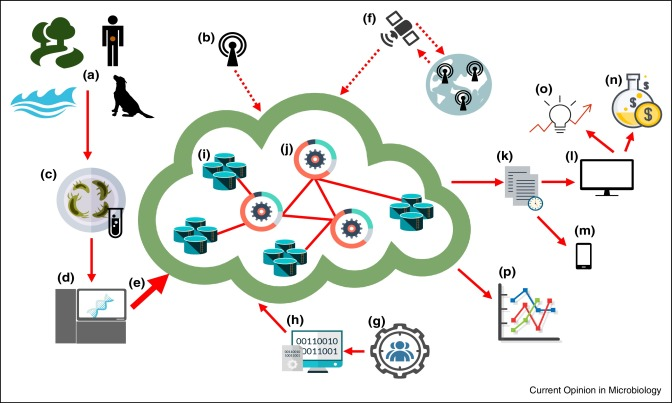
\includegraphics[width=\linewidth]{microbiome.png}
\end{frame}

\begin{frame}
  \frametitle{Microbiome study aims}
  \centering
  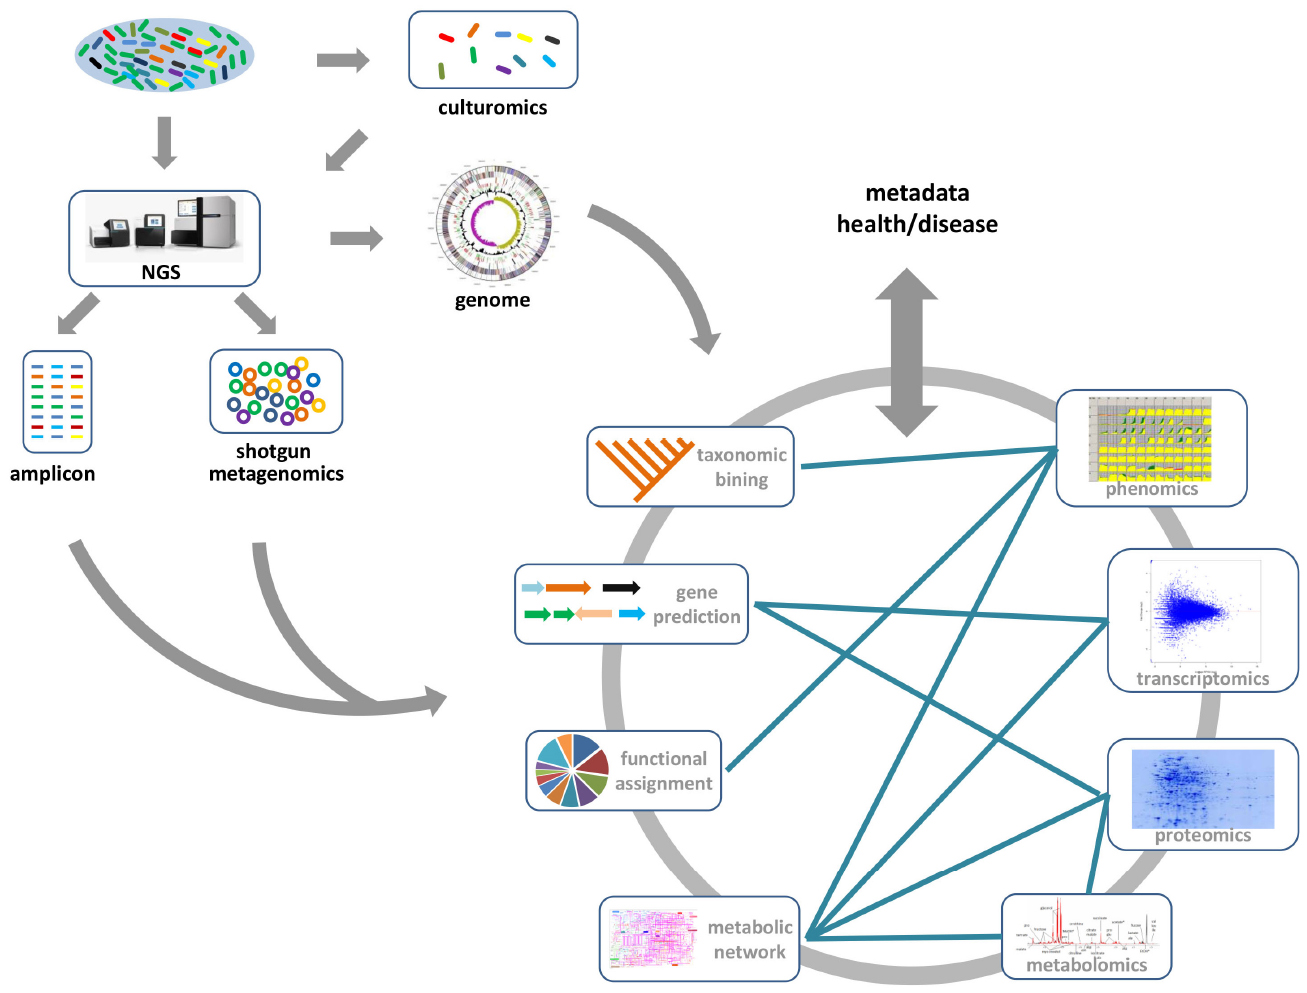
\includegraphics[width=\linewidth]{microbiome-study.png}
\end{frame}

\begin{frame}
  \frametitle{Microbiome study process}
  \centering
  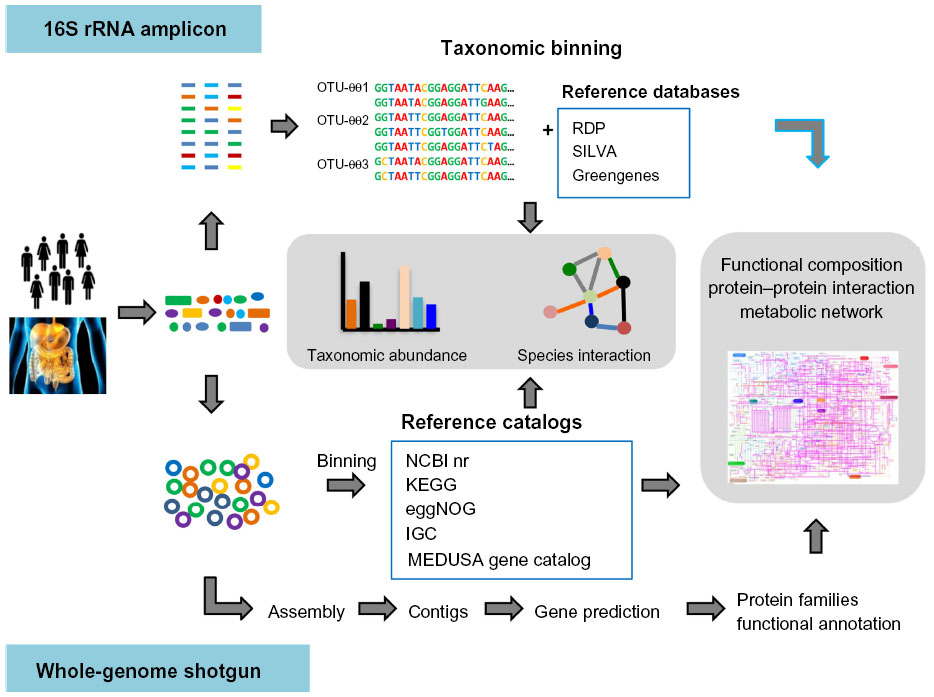
\includegraphics[width=\linewidth]{microbiome-study2.png}
\end{frame}

\begin{frame}
  \frametitle{The aim of the research and development}

  The object of the research is genetic data processing. We would like to involve biologists in it. The subject is the amplicon data processing with MiSeq SOP\footnote{Standard Operational Procedure} (a technique).

  The primary \textbf{aim} of the research is to construct infrastructure which comprises
  \begin{itemize}
  \item Big Data database for sequence storage;
  \item metadata storage and adapters;
  \item visual construction of a processing model;
  \item cloud genetic data processing unit;
  \item metadata inference unit;
  \item data integration unit based on Semantic Web and Linked Open Data principles.
  \end{itemize}

\end{frame}

\begin{frame}
  \frametitle{The process of data analysis (MiSeq SOP)}
  \begin{enumerate}
  \item Reconstruct \emph{cotigs} (contiguous gene parts) from ``left'' and ``right'' \emph{readings}.
  \item Trim \textbf{bar-code} and other \emph{primers}.
  \item Filter sequences according to formal criteria (ambiguity, average length, maximal length of homopolymer).
  \item Classify \emph{unique} sequences and count their appearance in groups (samples).
  \item Alignment with reference sequences from SILVA database.
  \item Filter non-hanging sequences.
  \item Filter chimeras, fund unique sequences again.
  \item Classify sequences with respect to existing taxa hierarchy. Get \textbf{OTU}s.
  \end{enumerate}

  After these stages a large number of OTU\footnote{Operation Taxonomic Unit} classified has been obtained.

\end{frame}



\begin{frame}[fragile]
  \frametitle{Alignment (an example)}
{\tiny\ttfamily\begin{verbatim}
align.seqs(fasta=HXH779K01.shhh.trim.good.unique.fasta, reference=silva.bacteria.fasta)

HXH779K01.shhh.trim.good.unique.align
HXH779K01.shhh.trim.good.unique.align.report
HXH779K01.shhh.trim.good.unique.flip.accnos

summary.seqs(fasta=HXH779K01.shhh.trim.good.unique.align,
      count=HXH779K01.shhh.trim.good.count_table)

		Start	End	NBases	Ambigs	Polymer	NumSeqs
Minimum:	6237	22529	5	0	1	1
2.5%-tile:	6428	22577	409	0	4	835
25%-tile:	6428	25292	420	0	4	8349
Median: 	6428	25292	423	0	5	16697
75%-tile:	6428	25292	442	0	5	25045
97.5%-tile:	6430	25293	446	0	6	32558
Maximum:	43107	43116	476	0	9	33392
Mean:	6435	25061	429	0	4
# of unique seqs:	26744
total # of seqs:	33392

It took 21 secs to summarize 33392 sequences.
\end{verbatim}}
\end{frame}

\begin{frame}[fragile]
  \frametitle{OTU classification analysis (an example)}
{\tiny\ttfamily\begin{verbatim}

classify.otu(list=HXH779K01.shhh.trim.good.unique.good.filter.unique.precluster.pick.pick.opti_mcc.list,
 count=HXH779K01.shhh.trim.good.unique.good.filter.unique.precluster.denovo.vsearch.pick.pick.count_table,
 taxonomy=HXH779K01.shhh.trim.good.unique.good.filter.unique.precluster.pick.rdp.wang.pick.taxonomy,
 label=0.03)


OTU     Size    Taxonomy
Otu001  2883    Bacteria(100);Bacteria_unclassified(100);Bacteria_unclassified(100);
                Bacteria_unclassified(100);Bacteria_unclassified(100);Bacteria_unclassified(100);
Otu003  1038    Bacteria(100);"Actinobacteria"(100);Actinobacteria(100);Actinomycetales(100);
                Actinomycetales_unclassified(100);Actinomycetales_unclassified(100);
Otu005  660     Bacteria(100);"Actinobacteria"(100);Actinobacteria(100);Acidimicrobiales(100);
                Acidimicrobiaceae(99);Ilumatobacter(99);
Otu007  497     Bacteria(100);"Verrucomicrobia"(100);Subdivision3(100);Subdivision3_..._sedis(100);
                Subdivision3_..._unclassified(100);Subdivision3_genera_incertae_sedis_unclassified(100);
Otu008  484     Bacteria(100);"Bacteroidetes"(100);Flavobacteria(100);"Flavobacteriales"(100);
                Flavobacteriaceae(100);Flavobacterium(100);
\end{verbatim}}
  \begin{center}
  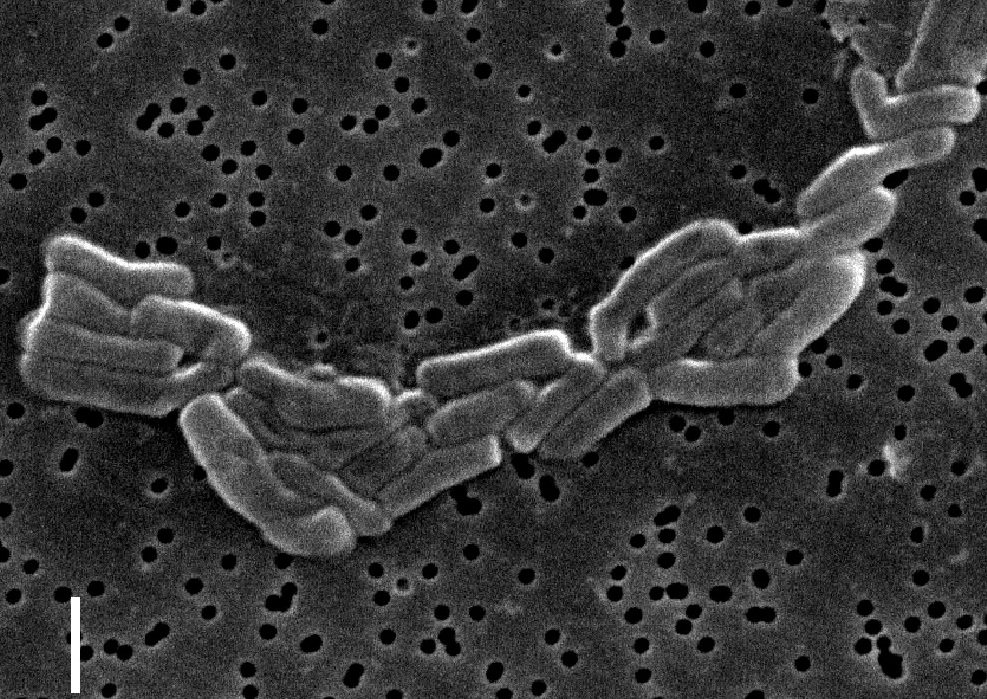
\includegraphics[width=0.4\linewidth]{illumatobacter.jpg} ${}$
  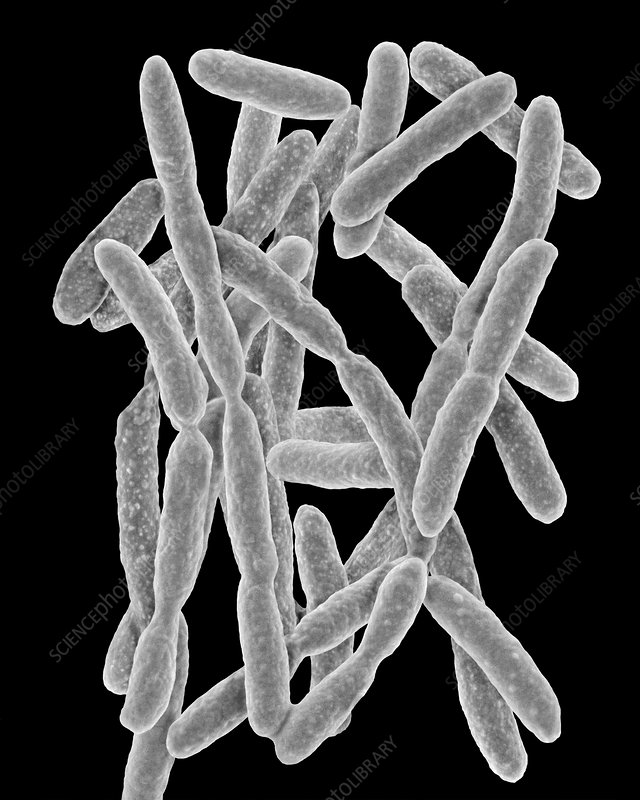
\includegraphics[width=0.3\linewidth]{flavobacter.jpg}
  \end{center}
\end{frame}

\begin{frame}
  \frametitle{Phylogenetic OTU investigations}
\centering
  \includegraphics[width=0.7\linewidth]{phylotree-proc.png}
% TODO: uncomment the prev line
\end{frame}

\begin{frame}
  \frametitle{A ``taxonomy'' of groups}
The taxonomy is build using unique sequences as a comparison basis. \\[2em]

\begingroup
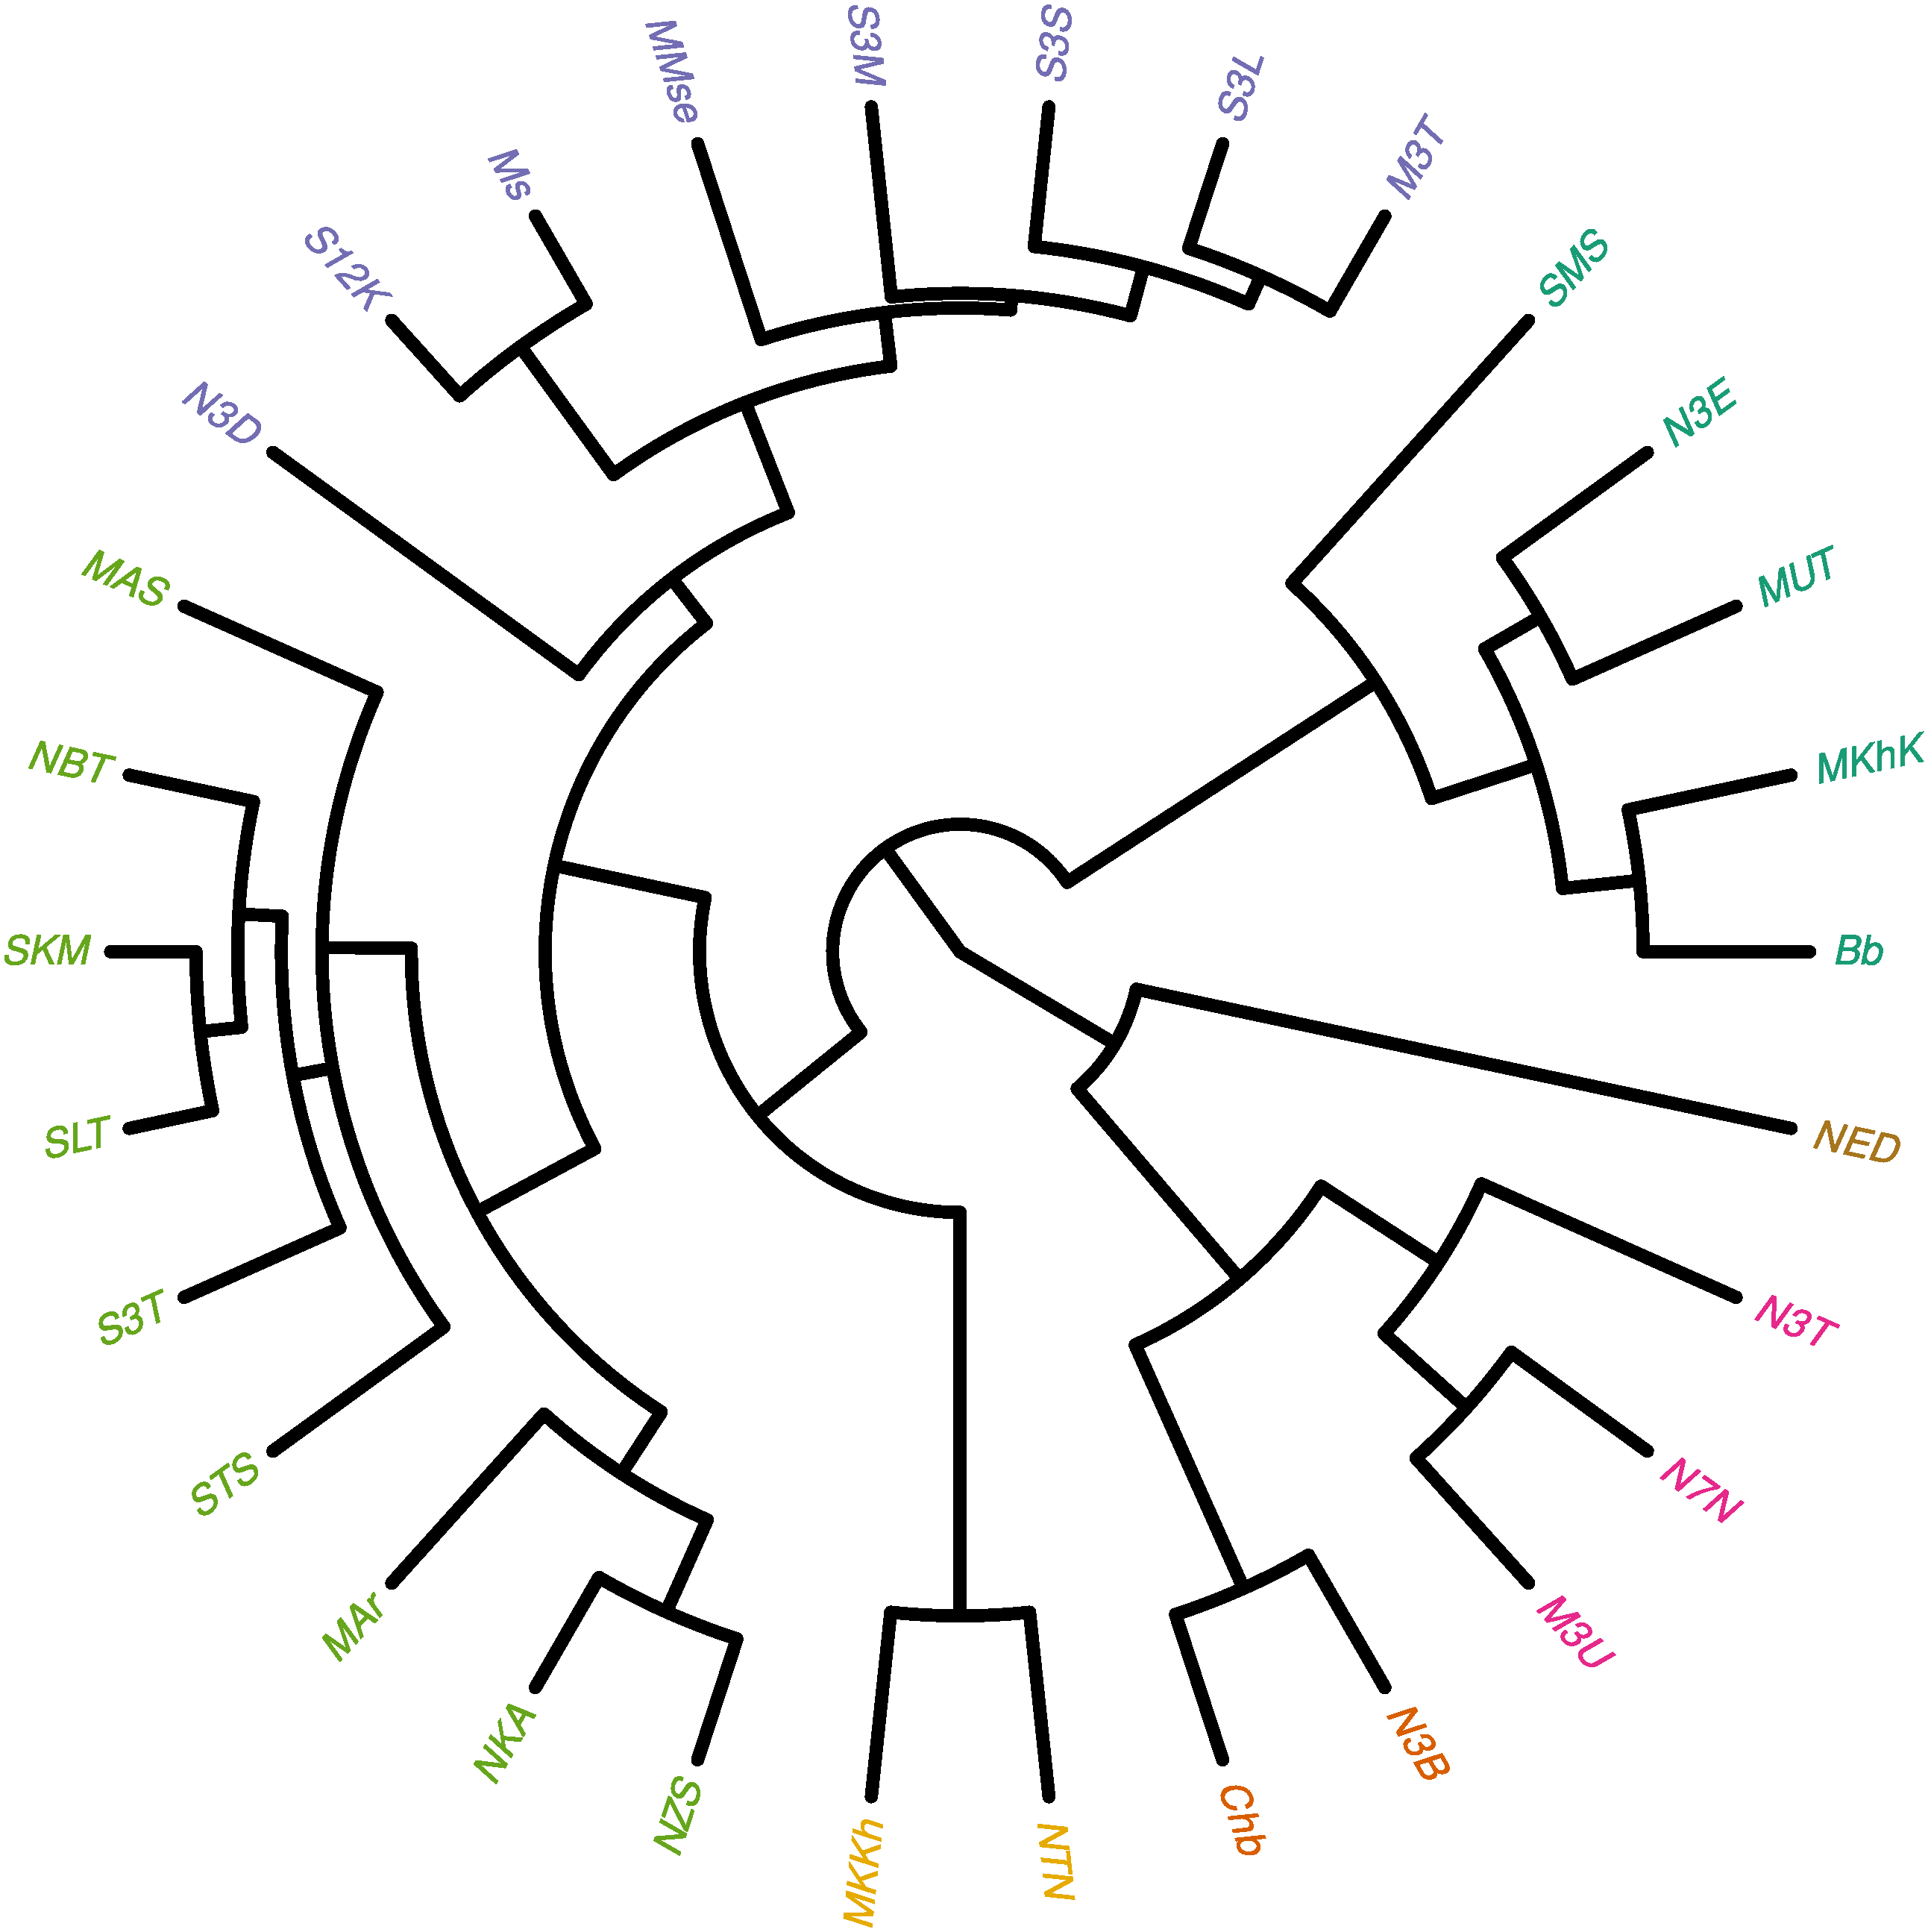
\includegraphics[width=0.5\linewidth]{probe-tree.pdf}\hfil
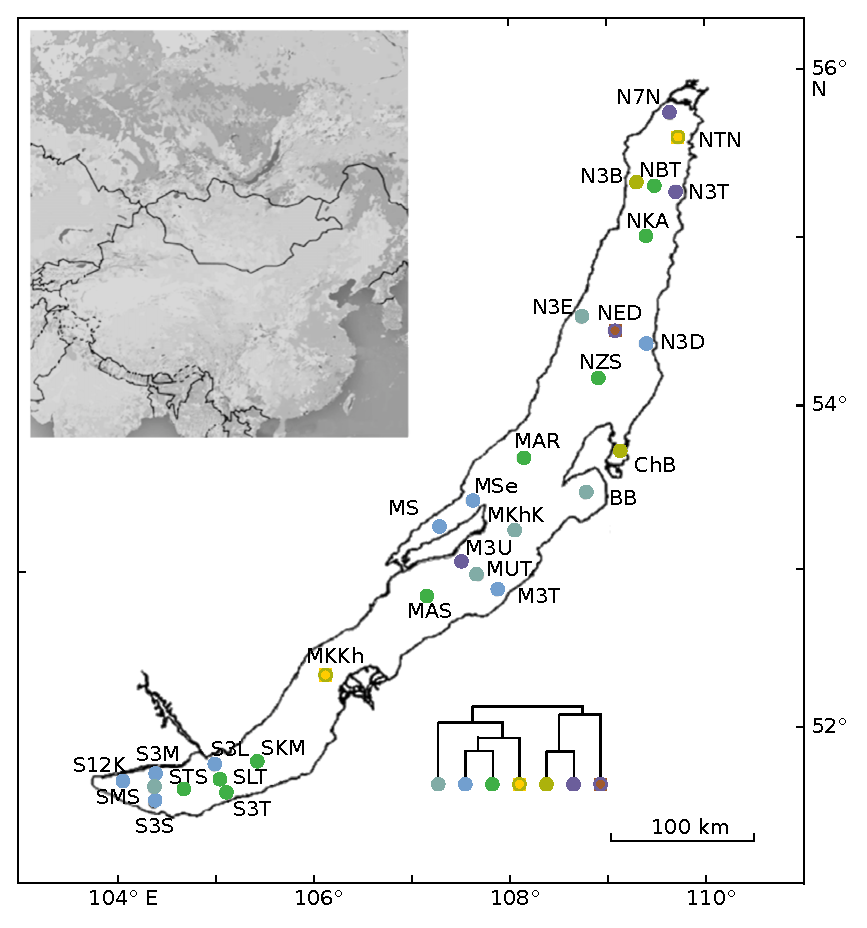
\includegraphics[width=0.45\linewidth]{baikal-probes.pdf}
\endgroup
\end{frame}

\begin{frame}
  \frametitle{Alpha-diversity}
\centering
  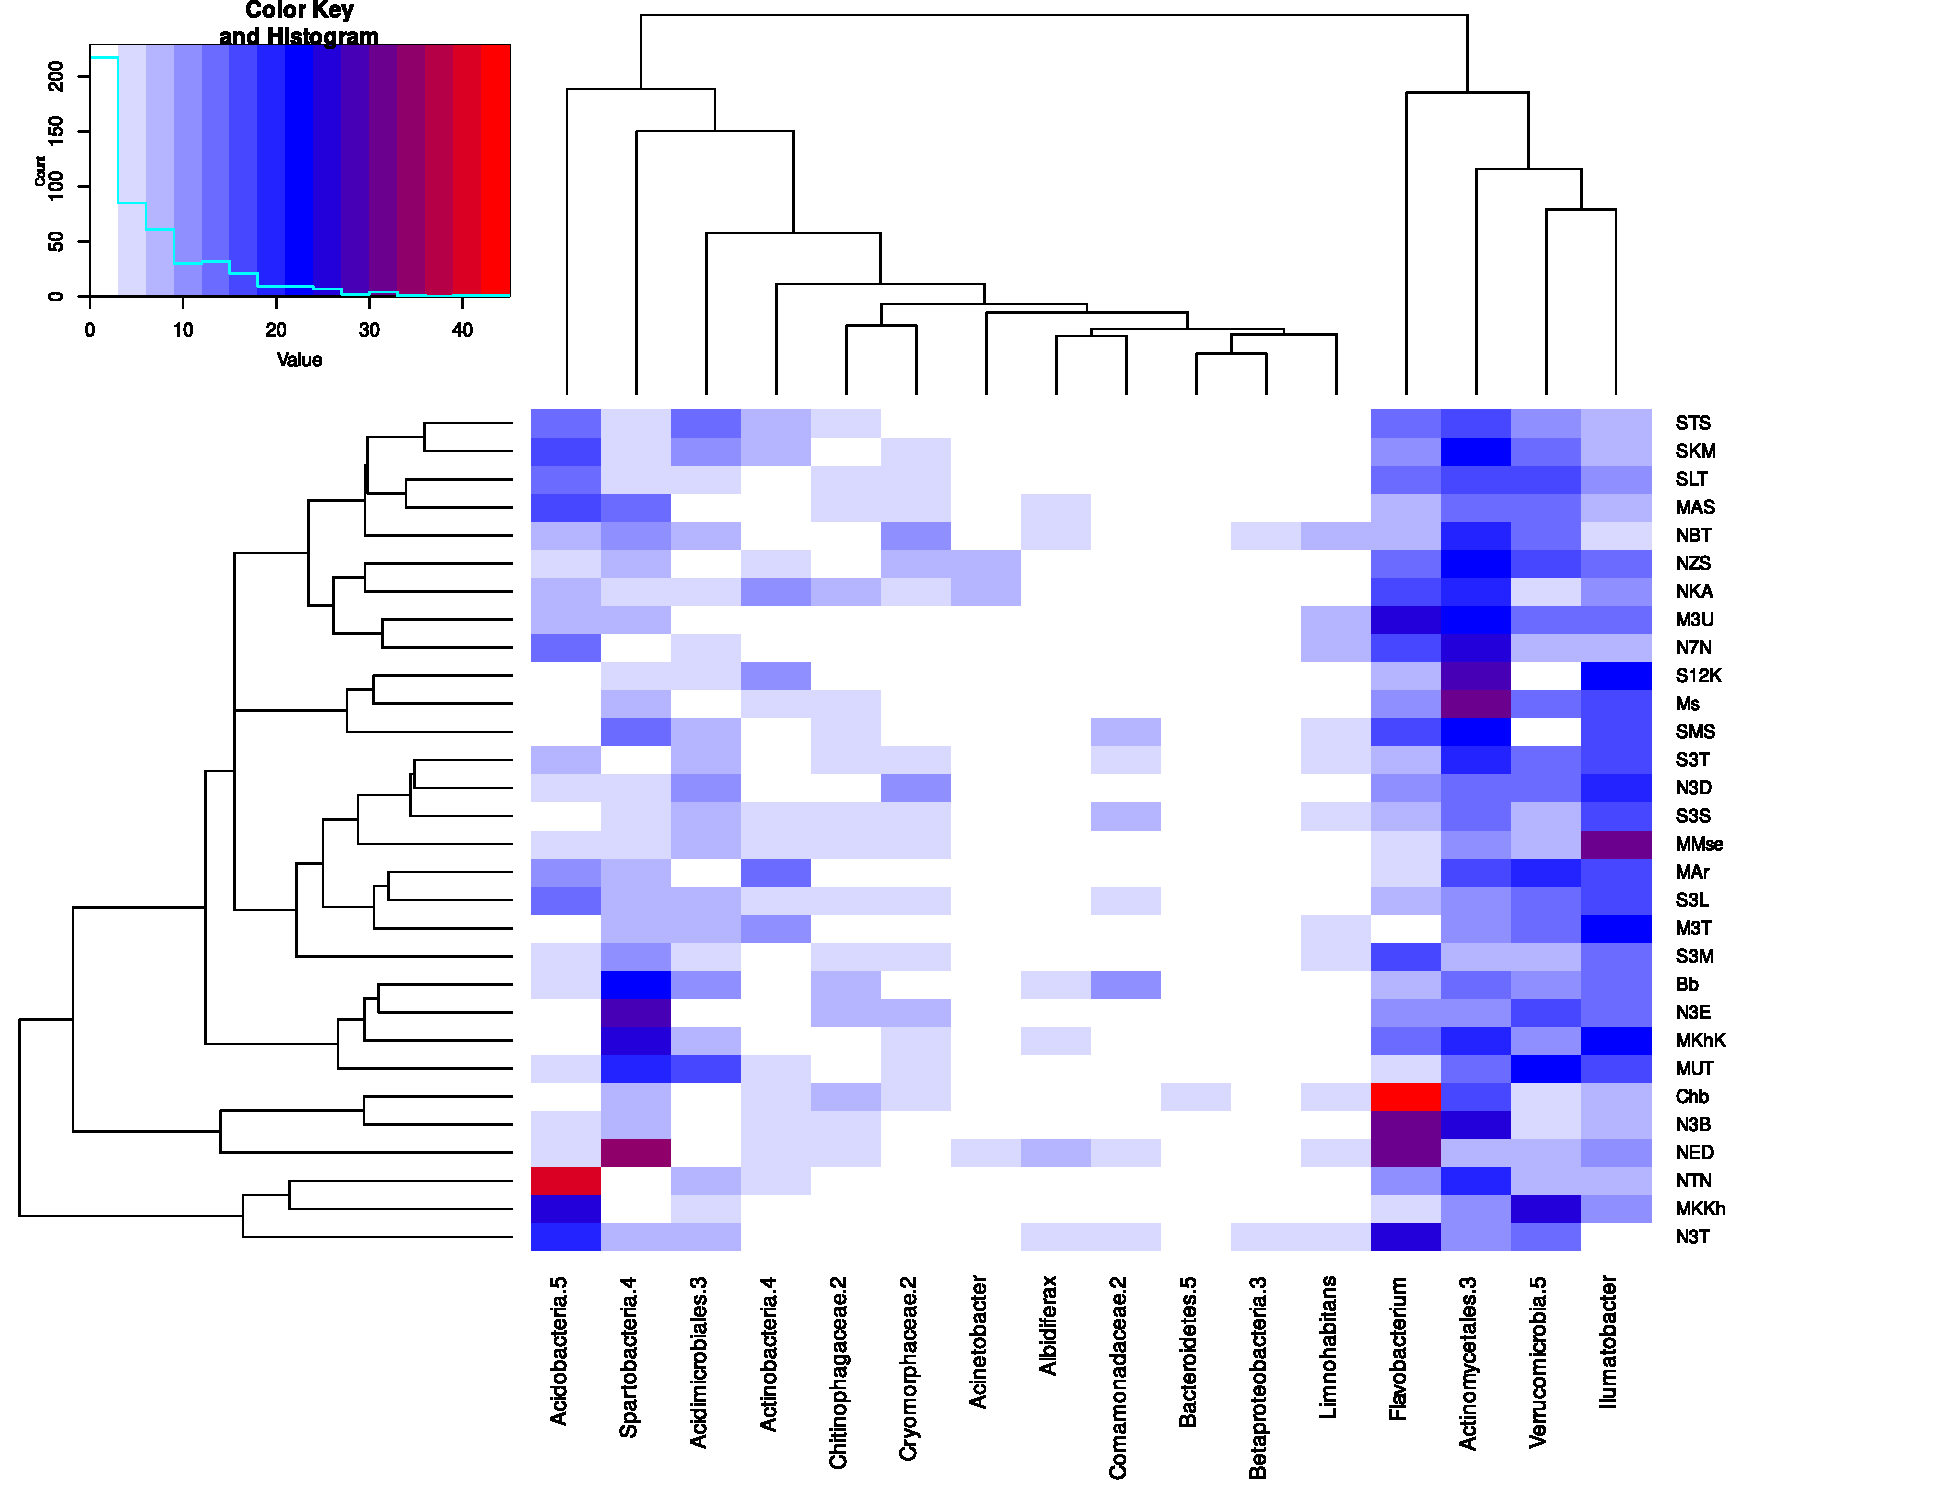
\includegraphics[width=1\linewidth]{heatmap-OTU-Group-tax.pdf}
\end{frame}

\begin{frame}
  \frametitle{Beta-diversity}
  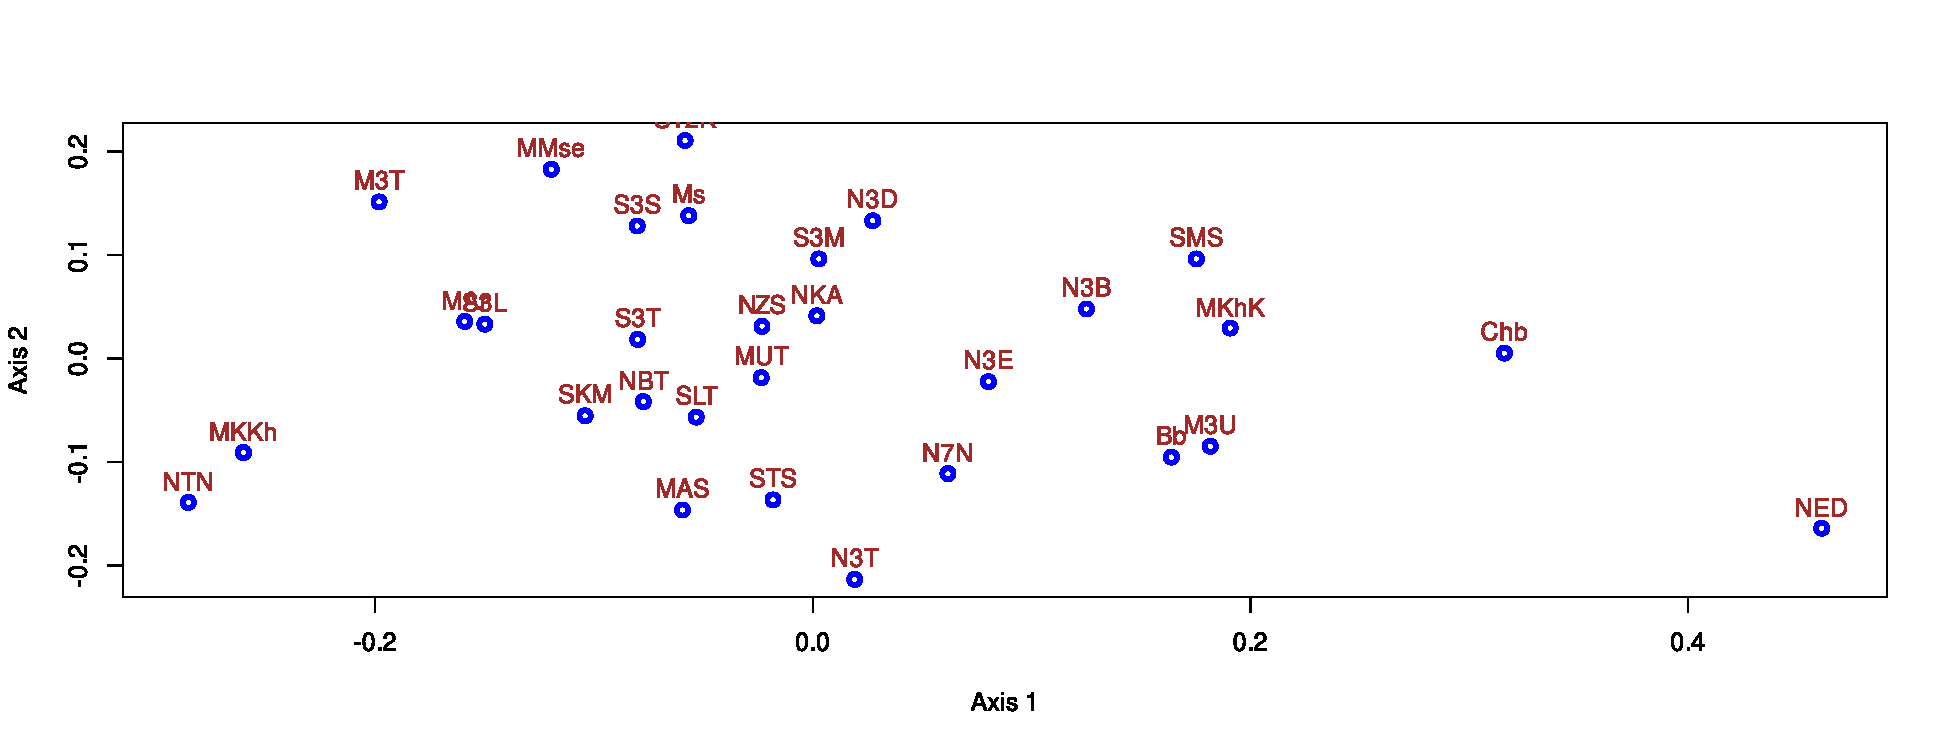
\includegraphics[width=1\linewidth]{nmds.pdf}
\end{frame}

\begin{frame}
  \frametitle{Dataflow representation of NGS analysis of amplicons}
  \begin{columns}
    \begin{column}{0.6\textwidth}
      \begin{raggedright}
        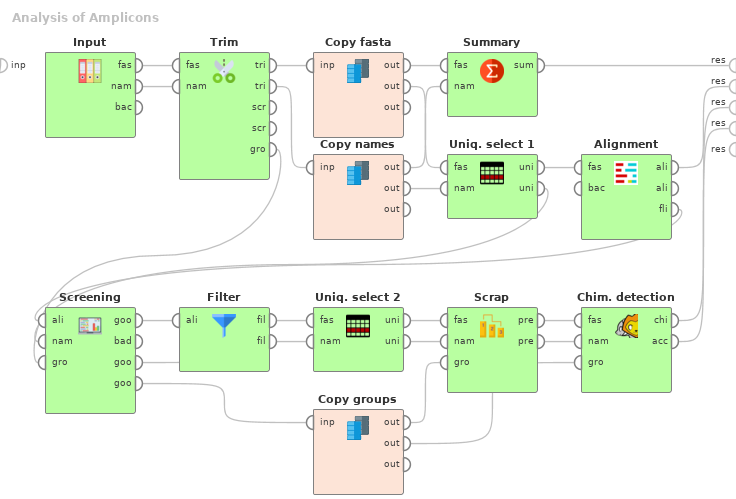
\includegraphics[width=1\linewidth]{Dataflow-color-en.png}
      \end{raggedright}
    \end{column}
    \begin{column}{0.4\textwidth}\footnotesize
      \begin{tabular}{ll}
        Term & Description \\
        \hline
        NGS & New Generation\\ & Sequencing\\
        Amplicon & A DNA or RNA part \\
                 & copied many times \\
        Mothur & A software toolset for\\ & NGS research \\
        Rapidminer & A visual tool for \\
             & data mining modeling\\
             &  and execution
      \end{tabular}
      ${}$\\[1em]
      Green blocks are Mothur modules. Others are Rapidminer modules.
    \end{column}
  \end{columns}
\end{frame}

\begin{frame}[fragile]
  \frametitle{Rapidminer module}
\begin{minted}[fontsize=\tiny]{cpp}
vector<string> AlignCommand::setParameters(){ // PART OF MODULE SOURCE
try {
  CommandParameter ptemplate("reference", "InputTypes", "", "", "none", "none", "none","",false,true,true); parameters.push_back(ptemplate);
  CommandParameter pcandidate("fasta", "InputTypes", "", "", "none", "none", "none","fasta-alignreport-accnos",false,true,true); parameters.push_back(pcandidate);
  CommandParameter psearch("search", "Multiple", "kmer-blast-suffix", "kmer", "", "", "","",false,false,true); parameters.push_back(psearch);
  CommandParameter pksize("ksize", "Number", "", "8", "", "", "","",false,false); parameters.push_back(pksize);
  CommandParameter pmatch("match", "Number", "", "1.0", "", "", "","",false,false); parameters.push_back(pmatch);
// . . . . . . .
\end{minted}
\begin{minted}[fontsize=\tiny]{java}
package com.rapidminer.ngs.operator; // GENERATED JAVA MODULE
// imports

class MothurChimeraCcodeOperator extends MothurGeneratedOperator {
  private InputPort fastaInPort = getInputPorts().createPort("fasta");
  private InputPort referenceInPort = getInputPorts().createPort("reference");
  private OutputPort chimeraOutPort = getOutputPorts().createPort("chimera");
  private OutputPort mapinfoOutPort = getOutputPorts().createPort("mapinfo");
  private OutputPort accnosOutPort = getOutputPorts().createPort("accnos");

  public MothurChimeraCcodeOperator (OperatorDescription description) {
    super(description);
  }
  @Override
  public void doWork() throws OperatorException {
    super();
    // . . . . . .
  }
  @Override
  public List<ParameterType> getParameterTypes() {
    super();
        // . . . . . .
  }
  @Override
  public String getOutputPattern(String type) {
    if (type=="chimera") return "[filename],[tag],ccode.chimeras-[filename],ccode.chimeras";
    if (type=="mapinfo") return "[filename],mapinfo";
    if (type=="accnos") return "[filename],[tag],ccode.accnos-[filename],ccode.accnos";
    return super.getOutputPattern(type);
  }
}
\end{minted}
\end{frame}


\begin{frame}
  \frametitle{Model Driven Architecture and Linked Open Data}
  \begin{center}
    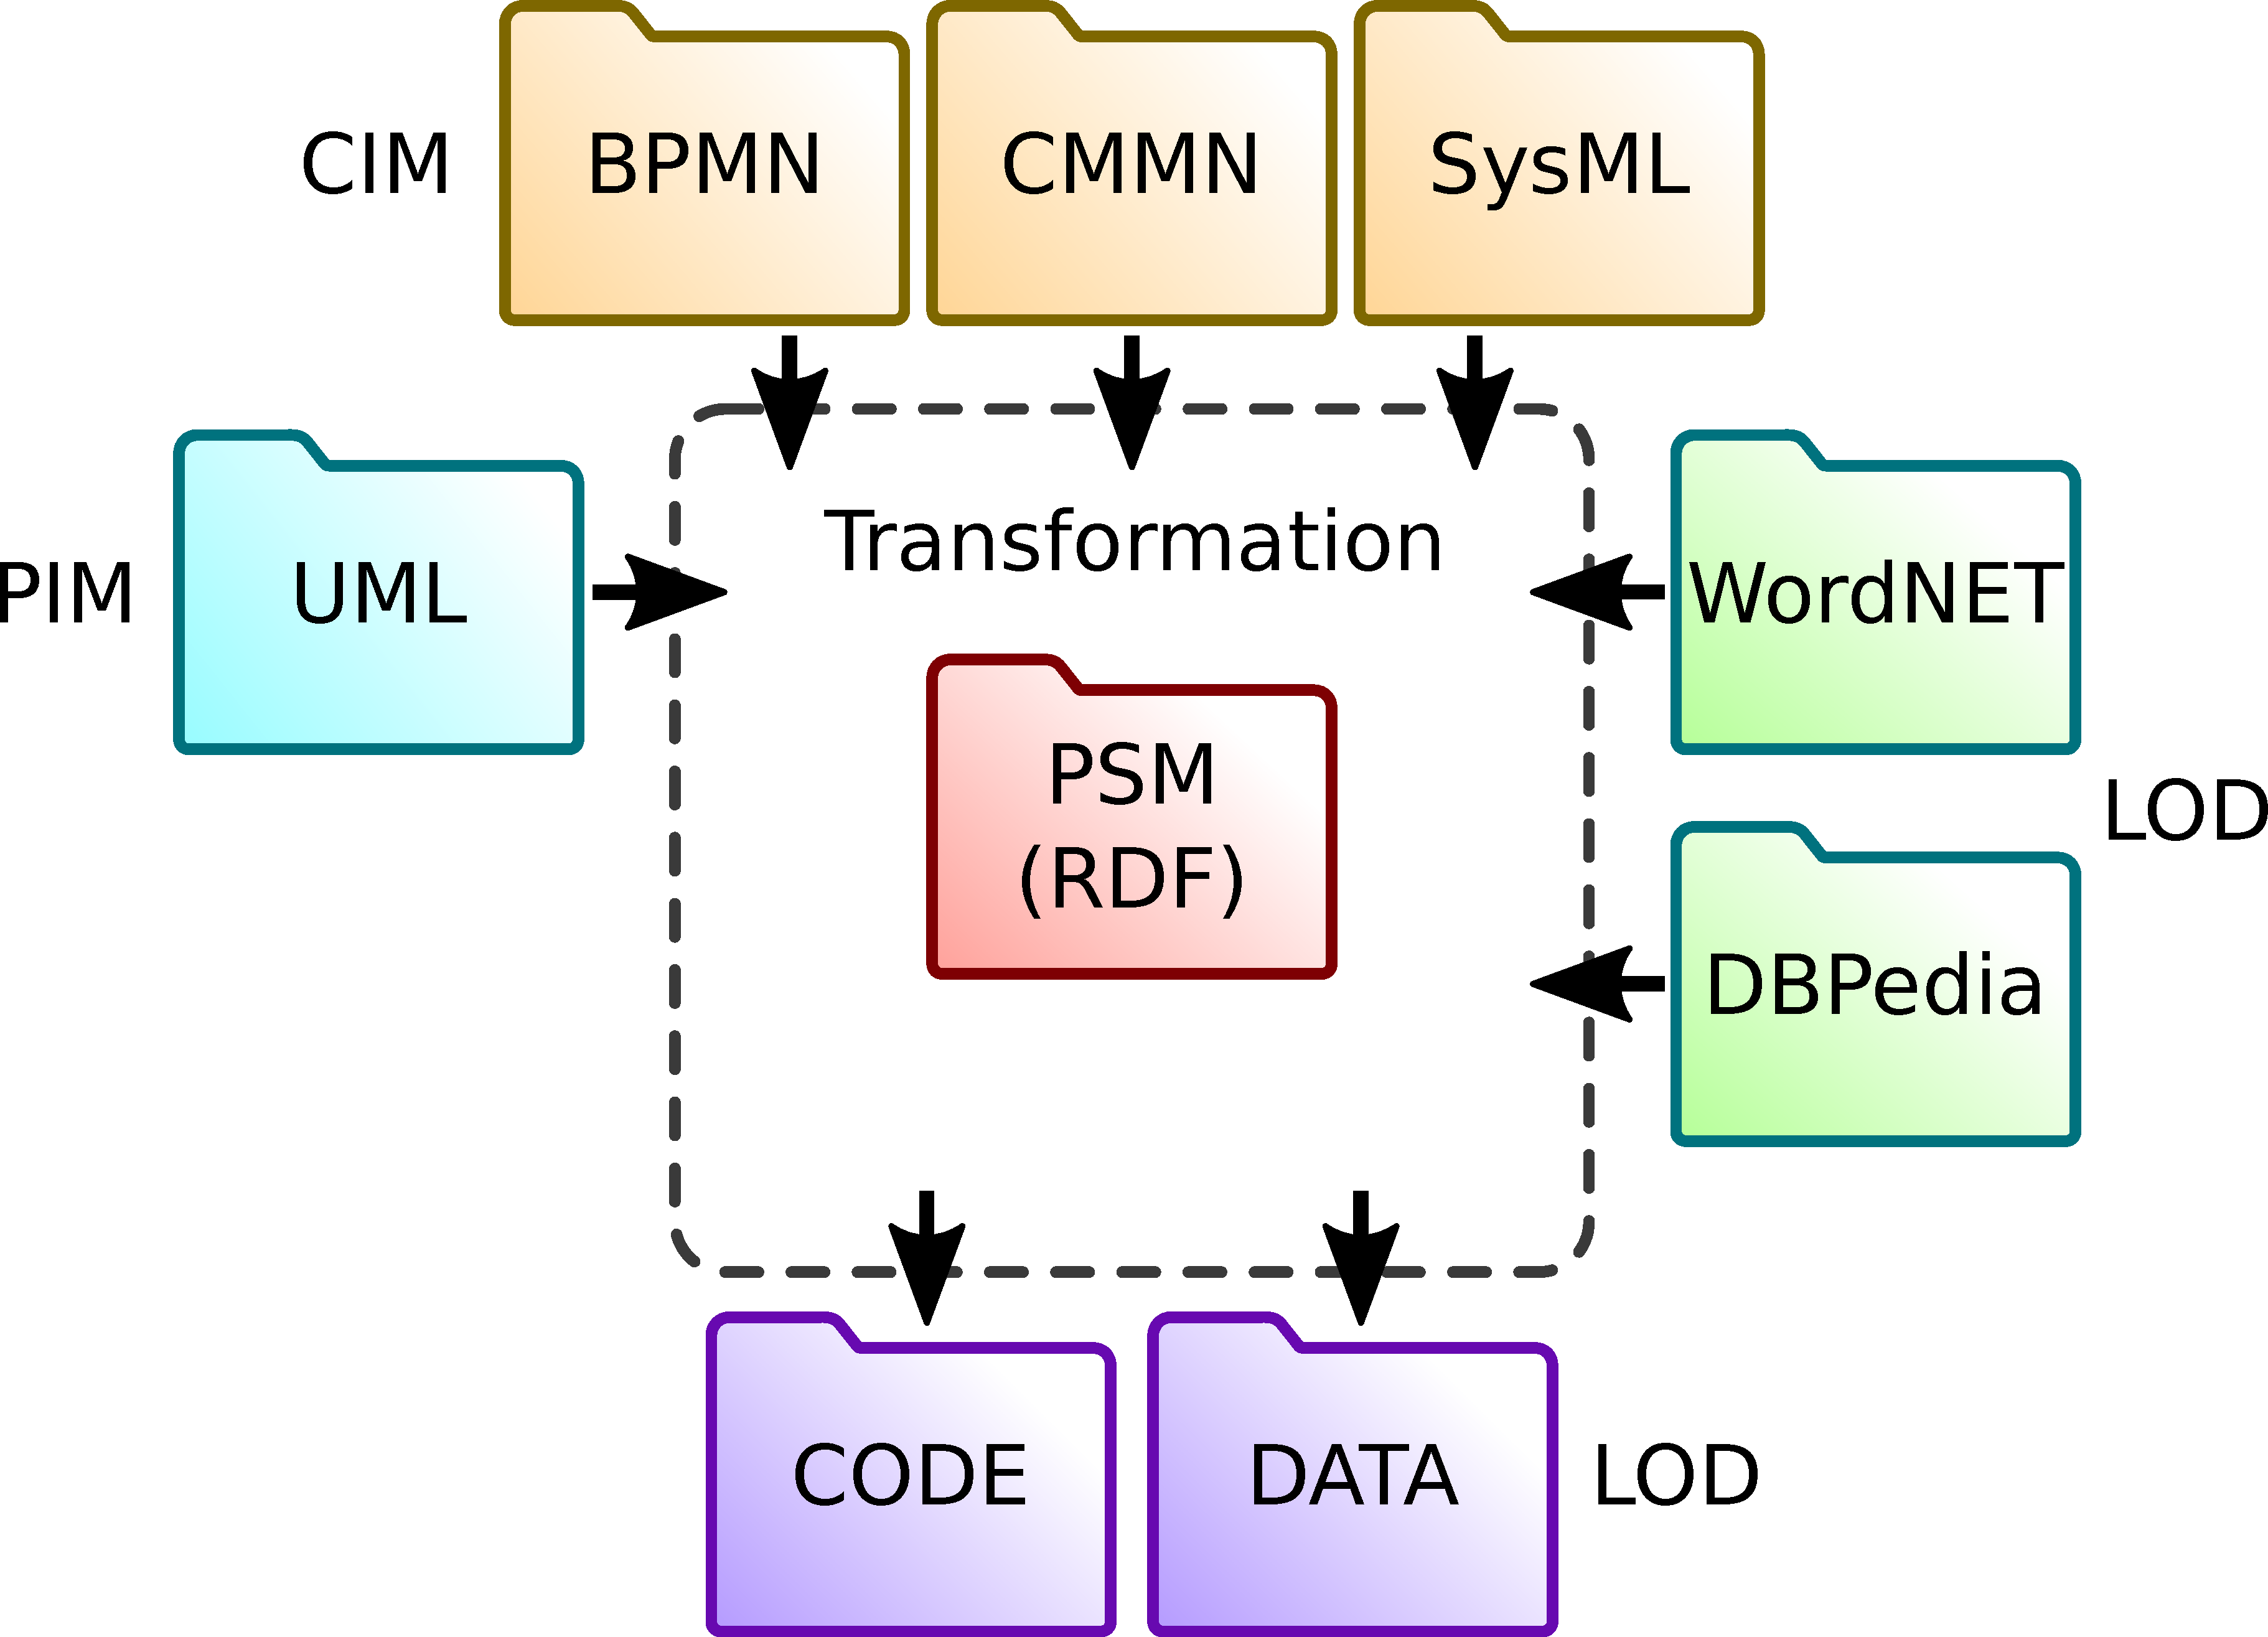
\includegraphics[width=0.9\linewidth]{mda-overview.pdf}
  \end{center}
\end{frame}

\begin{frame}
  \frametitle{MDA infrastructure}
  \centering
  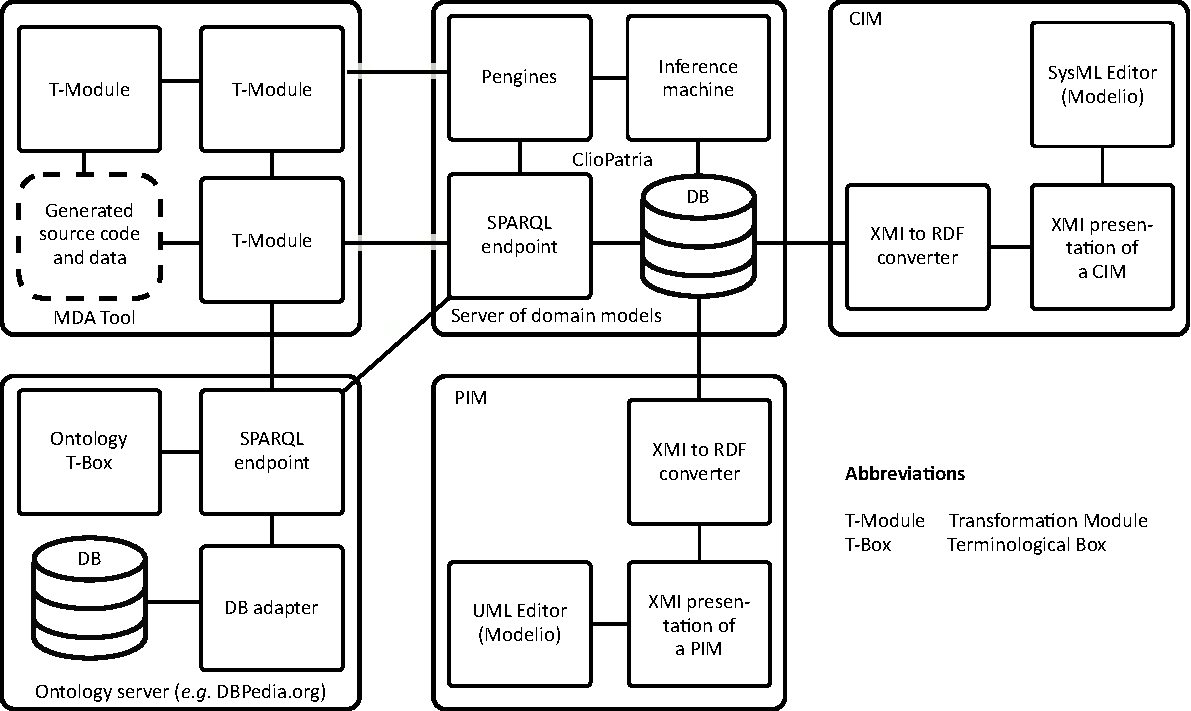
\includegraphics[width=1\linewidth]{architecture-mda-lod-ext.pdf}
\end{frame}

\begin{frame}
  \frametitle{Logtalk as transformation definition language}
  We have chosen Logtalk as it
  \begin{itemize}
  \item inherits widely known Prolog language syntax and runtime;
  \item implemented as macro package, performance penalties are about 1.5\%;
  \item has flexible semantics: we can define transformations and constraints within the same syntax;
  \item implement object-oriented knowledge (rules) structuring, encapsulation and replacement;
  \item compositional way of transformation implementation;
  \item powerful engine to post constraints on object-to-object messages (events);
  \item has implementation for many Prolog engines.
  \end{itemize}
  The <<regular>> language allow us to use its libraries not directly related to MDA transformations.
\end{frame}

\begin{frame}[fragile]
  \frametitle{Semantic Web technologies in representation of models
    during transformation}
  \begin{itemize}
  \item Assimilates experience of domain basic researches trending to standardization;
  \item Regular set of triples denote a graph (T-Box, A-Box);
  \item Standard vocabularies are formally described (\verb|rdfs:domain|, \verb|rdfs:range|);
  \item Supported with most programming systems (libraries, inference engines, SPARQL);
  \item RDF has a way of global element identification, \emph{i.e.} we can refer the same object from different software systems;
  \item SWI-Prolog supports direct queries to a graph, as well as interpreting some predicates (\verb|rdfs:label|, \verb|dc:title|), wraps sparse RDF structure into a predicate arguments; ontological server ClioPatria;
  \item There is simple way of data security implementation (\verb|rdfs:seeAlso|);
  \item By means of Semantic Web \& LOD we are able to organize data transfer between heterogeneous information systems.
  \end{itemize}
\end{frame}


\begin{frame}
  \frametitle{Used ontologies}

  Standardized ontologies

  \begin{itemize}
  \item Friend-of-a-friend (\textbf{foaf}) for agent information: individuals, legal entities, program agents.
  \item Provenance (\textbf{prov}) for making references between documents.
  \item Dublin Core (\textbf{dc}) for published resources metadata mark up.
  \item DBPedia resource (\textbf{dbr}) to refer external classes and instance objects.
  \item Schema.org (\textbf{schema}) for Google, Yandex, Yahoo, \emph{etc}. searchable objects, structural elements.
  \item The Bibliographic Ontology (\textbf{bibo}) used for literature reference mark up.
  \item Open annotation (\texttt{oa}) as an ``bookmark'' ontology.
  \end{itemize}

  Non-standard ontologies

  \begin{itemize}
  \item Ontology \texttt{nssp} for Mothur source code processing results.
  \item Ontology \texttt{uml} for XMI representation.
  \end{itemize}
\end{frame}



\begin{frame}
  \frametitle{Linked Open Data, LOD}
  \begin{enumerate}
  \item Information is published in Internet with open access license;
  \item It is represented in a machine-readable form, e.g., Excel table instead of a bitmap picture;
  \item An open format used, e.g., CSV instead of Excel;
  \item The format is based on W3C recommended standards, allowing RDF and SPARQL reference;
  \item Published data refer to objects, forming context.
  \end{enumerate}
  Thus, applications publish data as relations of objects (entities).
\end{frame}

\begin{frame}[fragile]
  \frametitle{RDF (TTL) representation and ad its query object}
%\begin{multicols}{2}
\begin{minted}[fontsize=\tiny]{turtle}
@prefix xml: <http://www.w3.org/XML/1998/namespace> .
@prefix xsd: <http://www.w3.org/2001/XMLSchema#> .
ngsp:spec a ngsp:Specification ;
    ngsp:module mothur:NoCommand,
        mothur:align-check,
        mothur:align-seqs,
# . . . . .
mothur:align-check a ngsp:Module ;
    ngsp:outputPattern [ a cnt:Chars ;
            ngsp:parameterName "type" ;
            ngsp:pattern [ ngsp:patternString
                    "[filename],align.check" ;
                    dc:identifier "aligncheck" ] ;
            cnt:chars # . . . .
# . . . . .
mothur:align-check-idir-parameter a ngsp:Parameter ;
    ngsp:important false ;
    ngsp:multipleSelectionAllowed false ;
    ngsp:optionsDefault "" ;
    ngsp:required false ;
    ngsp:type mothur:String ;
    dc:title "inputdir" .

mothur:align-check-map-parameter a ngsp:Parameter ;
    ngsp:important true ;
    ngsp:multipleSelectionAllowed false ;
    ngsp:optionsDefault "" ;
    ngsp:required true ;
    ngsp:type mothur:InputTypes ;
    dc:title "map" .

mothur:align-check-name-parameter a ngsp:Parameter ;
    ngsp:chooseOnlyOneGroup "namecount" ;
    ngsp:important false ;
    ngsp:multipleSelectionAllowed false ;
# . . . . .
\end{minted}
% \begin{minted}[fontsize=\tiny]{logtalk}
% :- object(queryparam(_RDF,_Parameter),
%           extends(ngsquerybase)).

% :- public(type/1).
% type(Type) :-
%     ::attr(type, Type).
% :- public(name/1).
% name(Name) :- ::attr(dc:title, literal(Name)).
% :- public(options/1).
% options(Value):- ::attr(options, Value).
% :- public(options_default/1).
% options_default(Value):-
%     ::attr(optionsDefault, Value).
% % . . . . . . . .
% :- public(multiple_selection_allowed/0).
% multiple_selection_allowed:-
%     ::bool_attr(multipleSelectionAllowed).
% :- public(required/0).
% required:-
%     ::bool_attr(required).
% :- public(important/0).
% important:-
%     ::bool_attr(important).
% :- protected(attr/2).
% attr(NS:Name, Value):-
%     ::ngs(RDF),
%     ::second(Parameter),
%     rdf_db::rdf_global_object(Value, V),
%     RDF::rdf(Parameter, NS:Name, V).
% attr(Name, Value):-
%     \+ Name=_:_,!,
%     ::ngs(RDF),
%     ::second(Parameter),
%     rdf_db::rdf_global_id(Value, V),
%     RDF::rdf(Parameter, ngsp:Name, V).
% % . . . . .
% :- end_object.

% \end{minted}
%\end{multicols}
\end{frame}

\begin{frame}[fragile]
  \frametitle{PSM: Scenario of a Class synthesis}

%\begin{multicols}{2}
  \begin{columns}
    \begin{column}{0.6\textwidth}
\begin{minted}[fontsize=\tiny]{logtalk}
:- object(direct(_Package,_LocalProf,_CodeProf)).    % Transformation driver object
:- public([tr/4,tr/3]).                              % Public interface of a class synthesis scenario
% . . . . . . . . . .
tr(class, Class, ClassID):- ::package(Package),      % Synthesize a class
    query(Package)::class(Name, ClassID),            % Query package structure in XMI
    create_object(Class,      % . . . . .            % Create a <<Class>> object
    create_object(Attributes, % . . . . .            % Create <<Attributes>> object
    create_object(Methods,    % . . . . .            % ...<<Methods>>.
    Class::name(Name),                               % Name the class.
    % Generate attributes of the class,
    % organizing them in a local database.
    % ...methods...
    Class::attributes(Attributes),                   % Set the attributes for class.
    Class::methods(Methods).                         % ...methods.

tr(attribute, Attribute, ClassID, AttributeID):-     % Attribute transformations
    ::package(Package),
    query(Package)::attribute(Name,ClassID,AttrID),
    create_object(Attribute,  % . . . . .
    Attribute::name(Name).                           % Name the attribute.

tr(method, Method, ClassID, MethodID):-              % Transformation of methods
    ::package(Package),
    query(Package)::method(Name,ClassID,MethodID),
    create_object(Method,     % . . . . .
    Method::name(Name).                              % Name of the method
:- end_object.
\end{minted}
    \end{column}
    \begin{column}{0.4\linewidth}
      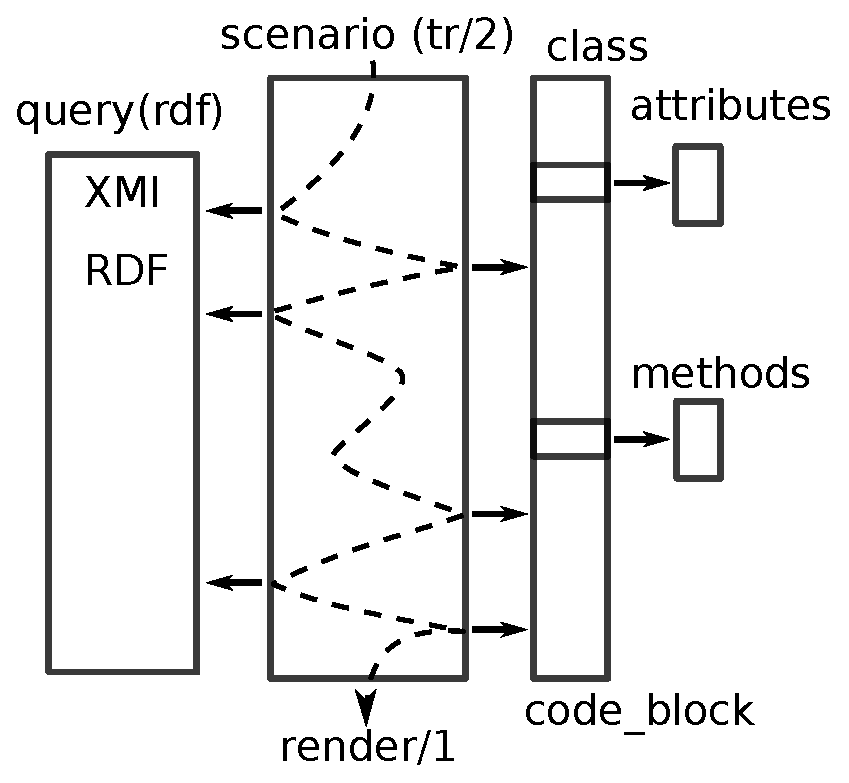
\includegraphics[width=1\linewidth]{scenario.pdf}
    \end{column}
  \end{columns}
  % \end{multicols}
\end{frame}

\begin{frame}[fragile]
  \frametitle{Implementation of \texttt{Query} object}
\begin{minted}[fontsize=\footnotesize{}]{logtalk}
:- object(query(_XMI)).
:- protected(xmi/1).
:- public([class/2, attribute/3, method/3]).
xmi(XMI) :- parameter(1, XMI).
class(Name, ID):-                            % Recognition of Class in RDF
    ::xmi(XMI),
    XMI::rdf(ID,rdf:type,uml:'Class'),
    XMI::rdf(ID,rdfs:label, literal(Name)).
attribute(Name, ClassID, ID):-               % ...attribute...
    ::xmi(XMI),
    XMI::rdf(ClassID, xmi:ownedAttribute, ID),
    XMI::rdf(ID, rdfs:label, literal(Name)).
method(Name, ClassID, ID):-                  % ...method...
    ::xmi(XMI),
    XMI::rdf(ClassID, xmi:ownedOperation, ID),
    XMI::rdf(ID, rdfs:label, literal(Name)).
% . . . . . . . . . . .
:- end_object.
\end{minted}
\end{frame}

\begin{frame}[fragile]
  \frametitle{Code Block (idea is taken from \texttt{llvmlite}${}^*$)}
  \begin{columns}
    \begin{column}{0.6\textwidth}
      \flushleft
\begin{minted}[fontsize=\footnotesize{}]{logtalk}
:- object(code_block, specializes(root)).
% Public interface of the object
:- public([append/1, prepend/1, clear/0,
   render/1, render_to/1, remove/1,
   item/1, items/1]).
% Code block items
:- dynamic([item_/1]).
:- private([item_/1]).
% Methods specialized during inheritance
:- protected([renderitem/2, render_to/2]).
% . . . . . . . . . . . .
% Delegate rendering to object itself
renderitem(Object, String):-
    current_object(Object), !,
    Object::render(String).
% Convert a literal to its string
% representation
renderitem(literal(Item), String):-!,
    atom_string(Item, String).
% Just print the item (debugging).
renderitem(Item, String):-
    root::iswritef(String, '%q', [Item]).
:- end_object.
\end{minted}
    \end{column}
    \begin{column}{0.4\textwidth}
      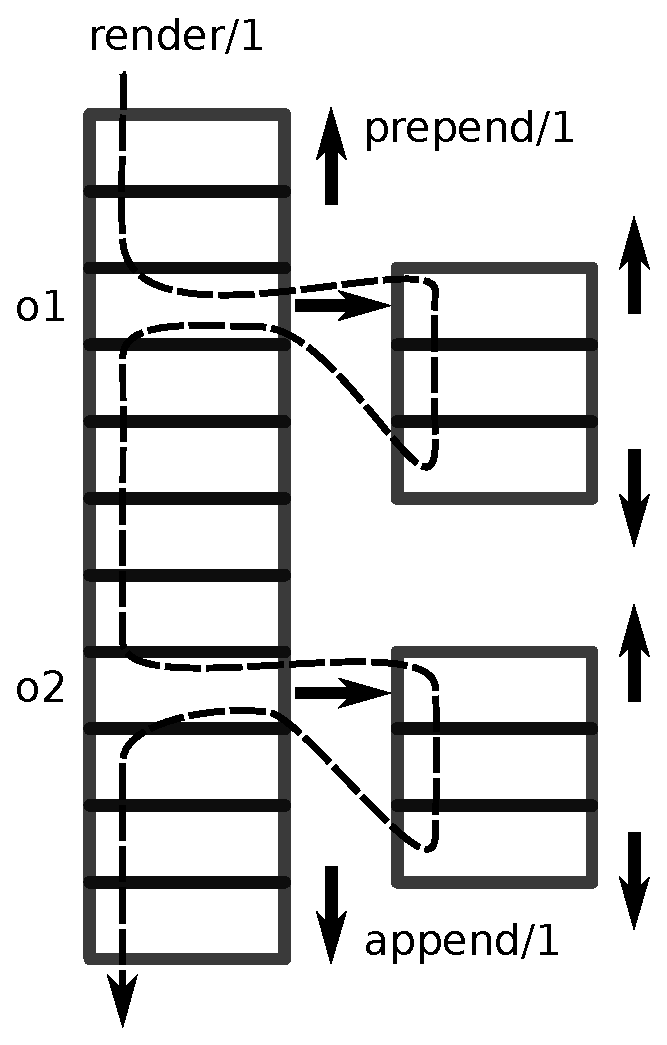
\includegraphics[width=1\linewidth]{code_block.pdf}
  ${}^*$) \url{https://github.com/numba/llvmlite}
    \end{column}
  \end{columns}
\end{frame}

\begin{frame}[fragile]
  \frametitle{PSM of a Python Class as a specialization of Code Block}
%\begin{multicols}{2}
  \begin{columns}
    \begin{column}{0.6\textwidth}
      \flushleft
\begin{minted}[fontsize=\scriptsize]{logtalk}
:- object(class, specializes(code_block),
   imports([named])). % Category of named entities
:- public([classlist/1, methods/1, attributes/1]).
% . . . . . . . . . . . . . .
renderitem(Item, Result):-      % proceed with default
    ^^renderitem(Item, Result). % rendering
render(Result):-         % Source generator
    ^^render(Name),      % implemented in a category
    ( ::item(classlist(List)) ->
     % . . . . . . . . . . .
        [Name]) ),
    ( ::item(attributes(Attributes))->
     % . . . . . . . . . . .
        [DefAttrList]),
      Attributes::items(InstanceAttrs),
      findall(S, ( % initialize attributes
         % . . . . . . . . .
         ), AttrAssigns),
        root::unindent,
        AttrList=[ConstructorDef|AttrAssigns];
         % . . . . . . . . .
        AttrList=[ConstructorDef, Pass] ),
    ( ::item(methods(Methods))-> % If any ...
      Methods::render(MethodList);
      MethodList=[] ),
    lists::append(AttrList,MethodList,StringList),
    root::unindent, Result=[Signature|StringList].
:- end_object.
\end{minted}
    \end{column}
    \begin{column}{0.4\linewidth}
      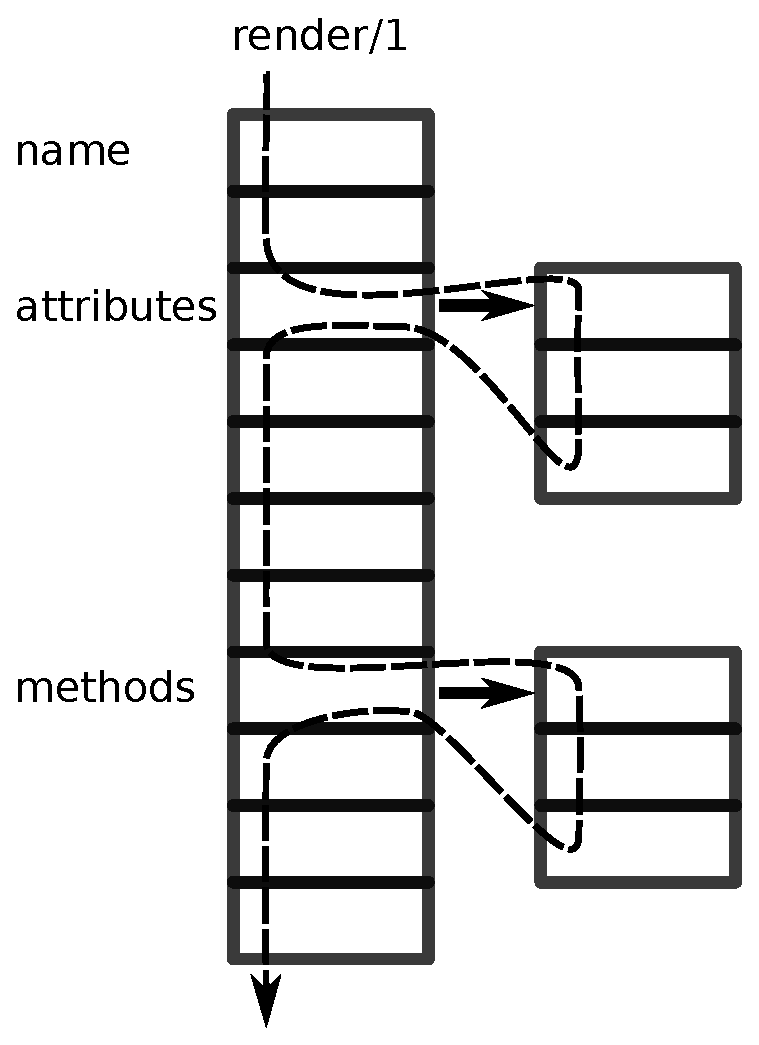
\includegraphics[width=1\linewidth]{code_block_class.pdf}
    \end{column}
  \end{columns}
  % \end{multicols}
\end{frame}

\begin{frame}[fragile]
  \frametitle{Logtalk Categories}
  A category of named entities
\begin{minted}[fontsize=\scriptsize]{logtalk}
:- category(named).
:- public([name/1, render/1]).
:- protected([renderitem/2]).
name(Name):- ::prepend(name(Name)).
renderitem(name(Name), String):-!, atom_string(Name, String).
render(String):-  % What is code generation from items
    ::item(name(Name)), ::renderitem(name(Name), String).
:-end_category.
\end{minted}
Category of named and typed entities
\begin{minted}[fontsize=\scriptsize]{logtalk}
:- category(namedtyped, extends(named)).
:- public([type/1,render/2, separator_option/2,list_separator/1]).
:- protected([renderitem/2]).
type(Type):- ::append(type(Type)).
renderitem(Item, String):- ^^renderitem(Item, String),!.
renderitem(type(Type),String):-!, ::list_separator(Separator),
    writef::swritef(String, '%w%w', [Separator, Type]).
render(Middle, String):- ^^render(SName),
    (   ::item(type(Type)) ->
        ::renderitem(type(Type), SType),
        string_concat(SName, Middle, _1),
        string_concat(_1, SType, String) ;
        SName = String  ).
render(String):-  ::render("", String).
list_separator(Separator):-
    ::separator_option(Name, Default),!, % Global options
    root::option(Name, Separator, Default).
:- end_category.

\end{minted}
\end{frame}

\begin{frame}
  \frametitle{Discussion (MDA application)}
  Interesting positive impressions obtained:
  \begin{itemize}
  \item Logtalk and RDF are flexible, sufficiently universal and convenient implementation infrastructures for MDA;
  \item The best implemenation means is Prolog predicate wrapping and Logtalk object encapsulation of rules;
  \item Not all Logtalk properties are investigated: there might be more sophisticated programming techniques developed, \emph{e.g.}, on the base of message watchers.
  \end{itemize}
  Technical problems making the approach somewhat problematic:
  \begin{itemize}
  \item Very simple tasks take too much efforts, \emph{e.g.}, text processing: convert an identifier into the CamelCase;
  \item It takes too long to surf Internet in order to find a vocabulary for a domain, but it is more productive than development new one and classes;
  \item Prolog is not a popular language in MDA, neither Logtalk.
  \end{itemize}
\end{frame}

\begin{frame}
  \frametitle{Future activities}
  The future activities supposed to be the follows:
  \begin{enumerate}
  \item Having dataflow models of MiSeq SOP and other techniques, device an intelligent subsystem, which will construct computational procedures for a predefined set of data processing tasks (\emph{AI's problem solving}).
  \item Implement a cloud or cluster computing environment for HPC processing the procedures.
  \item Create a more sophisticated source code parser or PIM model of computation so we will able to infer metadata for the output on the metadata of input.
  \item Realize adapters of data/metadata storage and retrieving, as well as the storage.
  \item Adapt our ``pattern-directed'' approach of semantically marked up document authoring to present input and output to the scientific communities.
  \item Implement integration to biological/gene databases.
  \item Write a handbook on Logtalk programming strategies with its author Paulo Mora.
  \end{enumerate}
\end{frame}

\begin{frame}
  \frametitle{Conclusion}
  The following results have been obtained as for today:
  \begin{itemize}
  \item A part of biologists' activities was investigated and patterns are described.
  \item A technique for interpretation of Mothur interfaces has been developed and implemented.
  \item Transformation tools are tested in application areas and no significant technical problems were detected.
  \item A technique of document authoring is being developed and adapted to the domain.
  \end{itemize}
  The source codes are available at \url{https://github.com/isu-enterprise/icc.xmitransform}, \url{https://github.com/eugeneai/icc.mothurpim}.

  This research is supported by Irkutsk scientific center of SB RAS, project No 4.2;
\end{frame}

\begin{frame}
  \frametitle{Technologies used (open source)}
  Python-3.x.x (\url{http://python.org}),\\
  ZCA (\url{https://muthukadan.net/docs/zca.html})\\
  SWIG (\url{http://swig.org/})\\
  SWI-Prolog (\url{https://www.swi-prolog.org/})\\
  Logtalk (\url{https://logtalk.org/})\\
  ClioPatria (\url{https://cliopatria.swi-prolog.org/home})\\
  Pengines (\url{https://pengines.swi-prolog.org/docs/index.html})\\
  LOV (\url{https://lov.linkeddata.es/dataset/lov/})\\
  Elastic Search (\url{https://www.elastic.co/})\\
  Kyotocabinet (\url{https://fallabs.com/kyotocabinet/})\\
  DBPedia (\url{https://wiki.dbpedia.org/})\\
  Mothur (\url{https://mothur.org/})\\
  R (\url{https://www.r-project.org/})
\end{frame}

\begin{frame}
  \frametitle{External links}
  \begin{columns}
    \begin{column}{0.5\textwidth}\centering
      
\includegraphics[width=1\linewidth]{qr-presentation.png}
      This presentation
    \end{column}
    \begin{column}{0.5\textwidth}\centering
      
\includegraphics[width=0.95\linewidth]{qr-illumina.png}
      Illumina movie on NGS
    \end{column}
  \end{columns}
\end{frame}

\begin{frame}
  \begin{center}
  \Large Thanks for Your interest to our project!
\end{center}
\end{frame}

\begin{frame}
  \frametitle{Architecture of transformation modules}
  \centering
  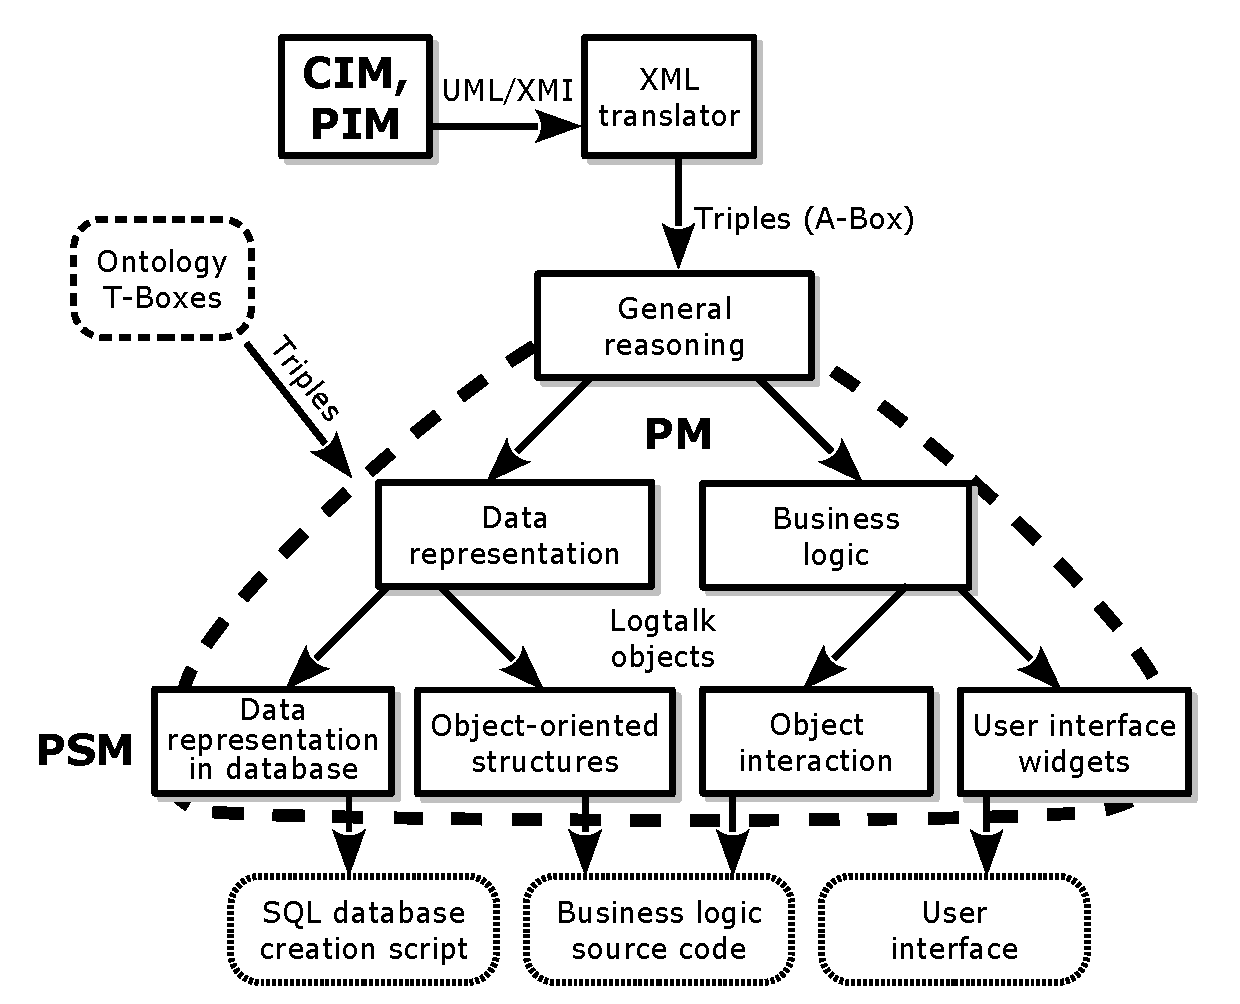
\includegraphics[width=0.9\linewidth]{architect_tree_pres-en-wo-OCL.pdf}
\end{frame}

\begin{frame}[fragile]
  \frametitle{Access LOD data}

  \begin{columns}
\begin{column}{0.5\textwidth}
\begin{minted}[fontsize=\scriptsize]{logtalk}
:- category(sparql).
:- public(query/2).
query(Pattern,Parameters,Row):-
    prepare(Pattern,Parameters,Query),
    server(Host,Port,Path),
    sparql_query(Query, Row,
        [host(Host),port(Port),path(Path)]).
:- protected(server/3).  % must be implemented
                         % by a subclass.
:- protected(prepare/3). % prepares a query
% . . . . . . . . . .    %             string.
:- end_category.

:- object(dbpedia, extends(sparql)).
:- protected(server/3).
server('dbpedia.org',80,'/sparql').
:- public(entity_name/2).
entity_name(Entity,Language,Name):-
    query('select ?name where { '
          ' %w rdfs:label ?name. '
          'FILTER langMatches( lang(?label),'
          ' "%w" )}', [Entity, Language],
          row(Name)).
:- end_object.

% ?- dbpedia::entity_name(dbr:'Passport', 'ru', Name).
\end{minted}
\end{column}
\begin{column}{0.5\textwidth}
  \flushright
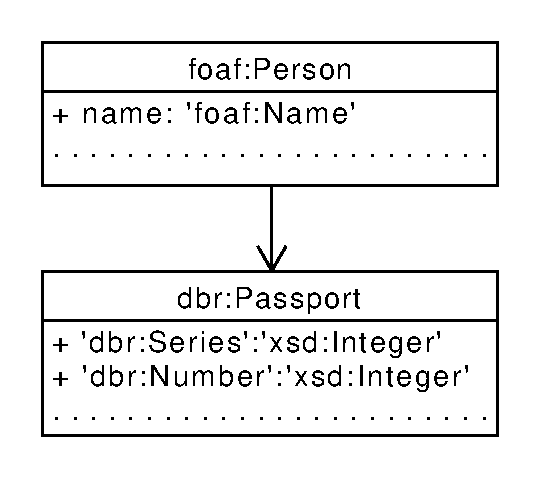
\includegraphics[width=0.8\linewidth]{simple-diag.pdf}
\end{column}
\end{columns}
\end{frame}

\begin{frame}
  \frametitle{Document authoring and storage}
  In most cases documents are created as a result of
  \begin{itemize}
  \item creative activity of a person with a text processors (authoring);
  \item printing a digital copy or a data record in a database;
  \item aggregation operation over database records (report).
  \end{itemize}
  Then it is stored either as a physical paper and/or a digital document (PDF, DOCX, HTML).

  Since 2000-th, Semantic Web and Linked Open Data (LOD) is being developed, allowing
  \begin{itemize}
  \item structural storage of data within published documents;
  \item processing stored data computationally;
  \item integration of data structures and data objects globally.
  \end{itemize}

  The \textbf{aim of this research} is to develop technologies, software and services allowing construction of digital archives supporting document data inclusion and inference from existing documents.
\end{frame}

\begin{frame}
  \frametitle{Structure of a document}
  \centering
  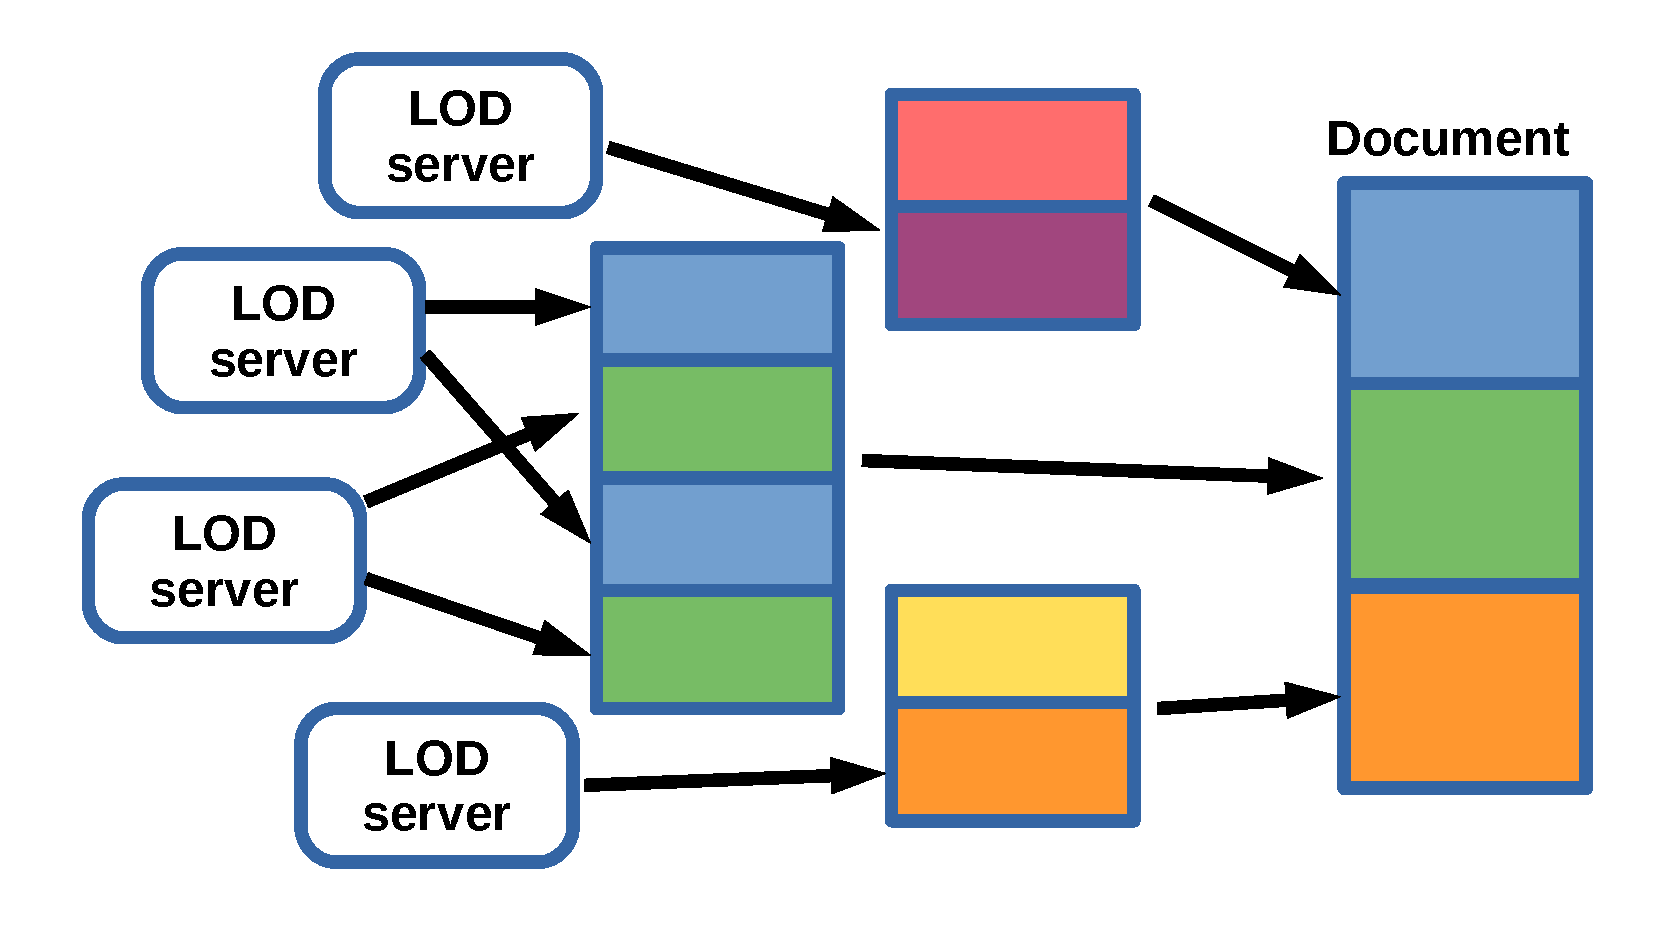
\includegraphics[width=1\linewidth]{document-structural-view.pdf}
\end{frame}

\begin{frame}
  \frametitle{Open Annotation (oa)}
\begin{adjustwidth}{-3em}{-3em}
  \centering
  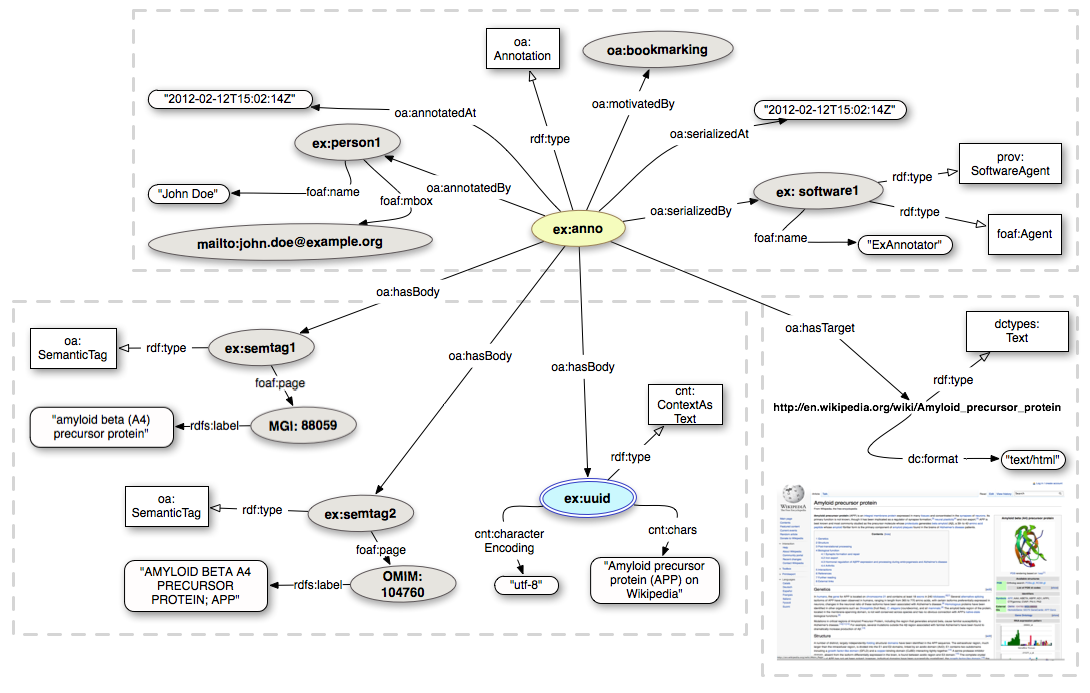
\includegraphics[width=1\linewidth]{Open-Annotation_CB_Bookmarking_and_Semantically_Tagging_A_webpage_spec20130128.png}
\end{adjustwidth}

\end{frame}

\begin{frame}[fragile,fragile]
  \frametitle{Representation}
  % \begin{block}{}
  %   \textbf{Целью} исследования является создание методики разработки процедур трансформации (PD\footnote{Platform [description] model.}) в виде ОО-модулей.
  % \end{block}
  % \begin{columns}
  %   \begin{column}{0.5\linewidth}
  %     % 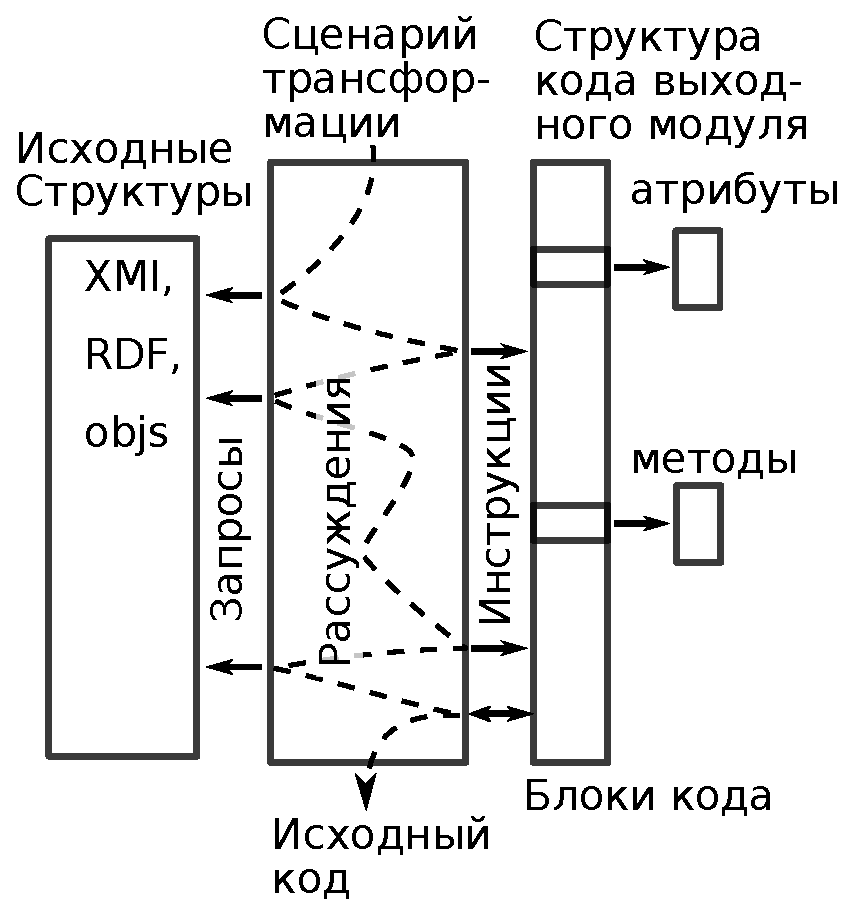
\includegraphics[width=1\linewidth]{pics/scenario-ru-wo-mothur.pdf}
  %   \end{column}
  %   \begin{column}{0.6\linewidth}
  %     Задачи исследования:
  %     \begin{itemize}
  %     \item Изучить синтаксические структуры Logtalk в аспекте структурирования знаний;
  %     \item Предложить методику представления трансформации в виде ОО-модулей;
  %     \item Реализовать библиотеку объектов и классов для МДА;
  %     \item Тестирование библиотеки на примере.
  %     \end{itemize}
  %   \end{column}
  % \end{columns}

\begin{adjustwidth}{-1.5em}{-1.5em}
\begin{minted}[escapeinside=||,fontsize=\btprgsize]{xml}
<html lang="ru" xmlns=http://www.w3.org/1999/xhtml
|\GB{xmlns:taa}|=http://irnok.net/engine/rdfa-manipulation
xml:lang="ru" metal:define-macro="page">
<head> . . . . </head>
<body prefix="rdf: http://www.w3.org/1999/...-ns# foaf: http://xmlns.com/foaf/...
imei: imei.html# course: https://irnok.net/college/plan/01..16-...\
%D0\%BA_PB-SM.plm.xml.xlsx-....2.3.1.html#"  resource="#post"
typeof="schema:CreativeWork sioc:Post prov:Entity">
<!-- The application control panel -->

<main lang="ru" resource="#annotation" typeof="oa:Annotation" id="main-doc-cnt">
<div property="oa:hasTarget" resource="#course-work-prog"></div>
<article property="oa:hasBody" typeof="foaf:Document curr:WorkingProgram"
         resource="#course-work-program" id="main-document">
  <div |\GB{taa:content}|="imei:title-page"></div>
  <div |\GB{taa:content}|="imei:neg-UMK"></div>
  <section id="TOC" class="break-after"> <h2>Table of Contents</h2>
    <div id="tableOfContents"></div>
  </section>
  <section id="course-description" resource="#description"
           property="schema:hasPart" typeof="schema:CreativeWork">
    <div property="schema:hasPart" resource="#purpose"
         typeof="dc:Text cnt:ContentAsText" >
      <div property="cnt:chars" datatype="xsd:string">
        <h2 property="dc:title" datatype="xsd:string">
           Aims and objectives of the discipline (module)</h2>
        <p>The aim of teaching the discipline ...</p>
      </div>
   </div>
  . . . . . . . .
\end{minted}
\end{adjustwidth}
\end{frame}

\begin{frame}
  \frametitle{Architecture}
  \begin{adjustwidth}{-2.5em}{-2.5em}
    \begin{center}
      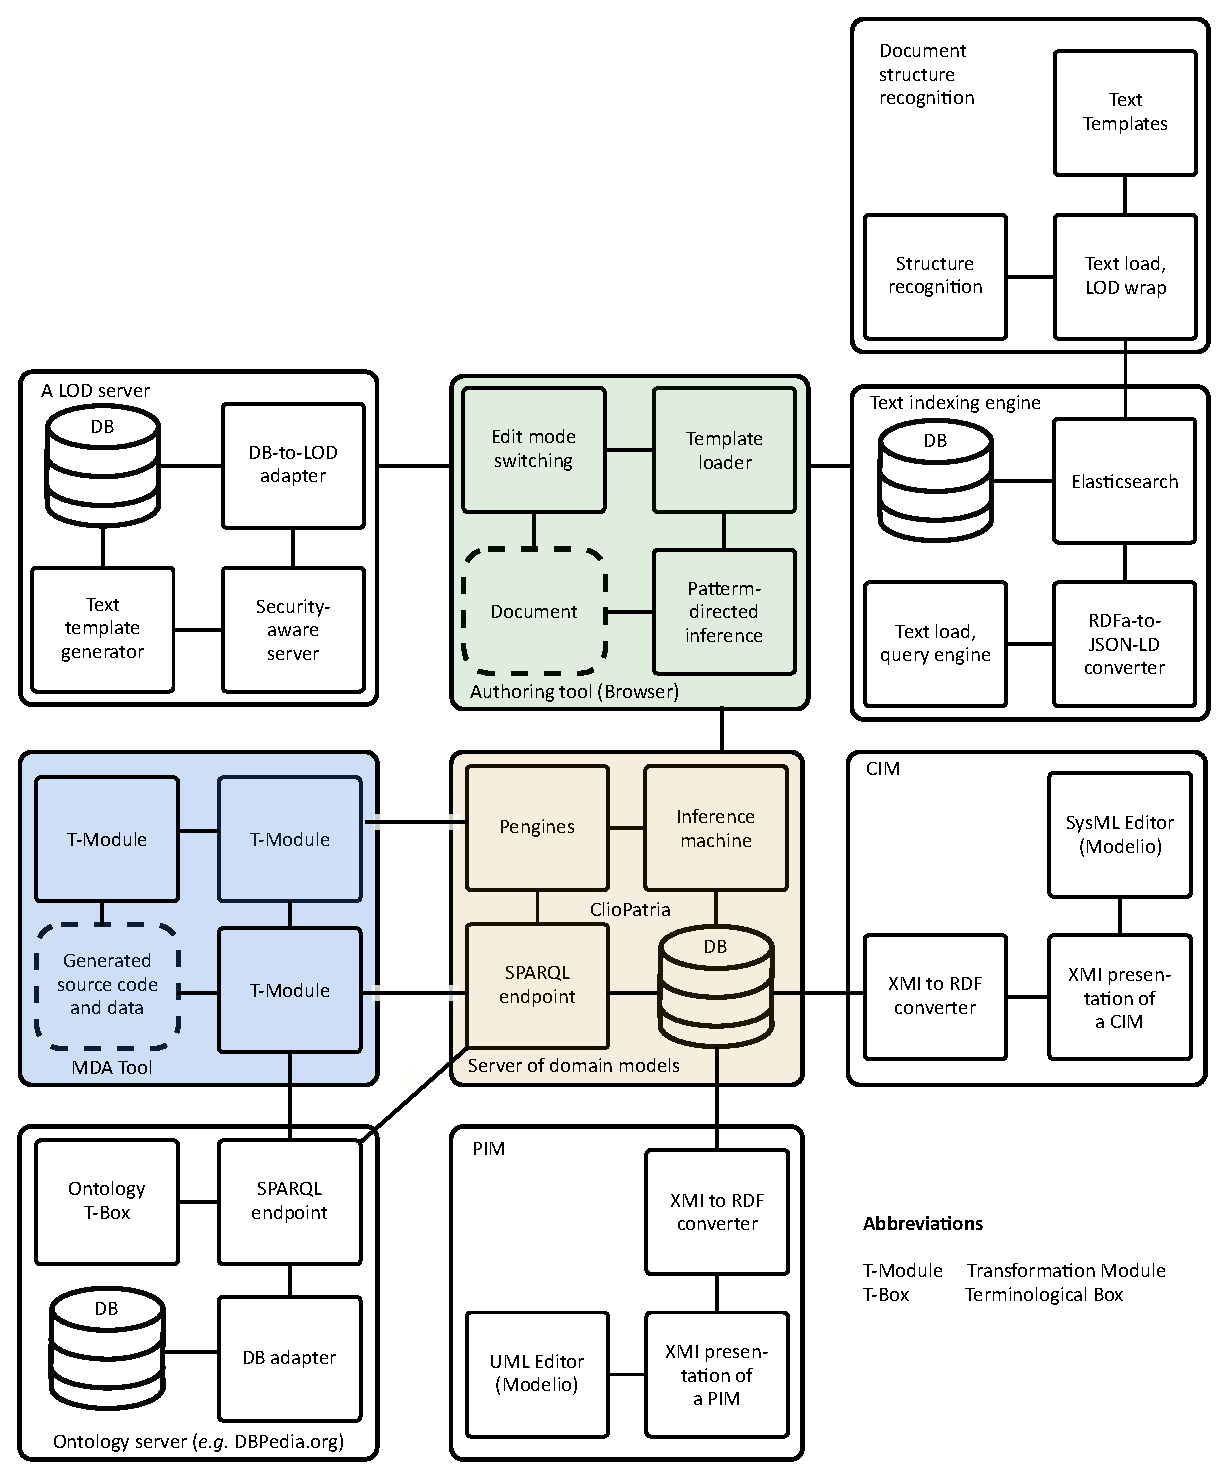
\includegraphics[width=0.5\linewidth]{architecture-mda-lod-ext-tot.pdf}
    \end{center}
  \end{adjustwidth}

% \begin{itemize}
% \item content and metadata repository with SPARQL (6) and full-text search (3); the engines for LOD processing (5) based on the logical inference;
% \item service for analysis of the stored content (2) enriching the archive with semantic information describing the content;
% \item tools for development of LOD applications and their user interfaces (1);
% \item browser based authoring tools (4).
% \end{itemize}
\end{frame}

\begin{frame}
  \frametitle{Generated list of title page preambles}
    \begin{adjustwidth}{-2.5em}{-2.5em}
    \begin{center}
      
\includegraphics[width=0.7\linewidth]{template-title-pages.jpg}
    \end{center}
  \end{adjustwidth}
\end{frame}

\begin{frame}
  \frametitle{Generated part of a study program}
   \begin{adjustwidth}{-2.5em}{-2.5em}
    \begin{center}
      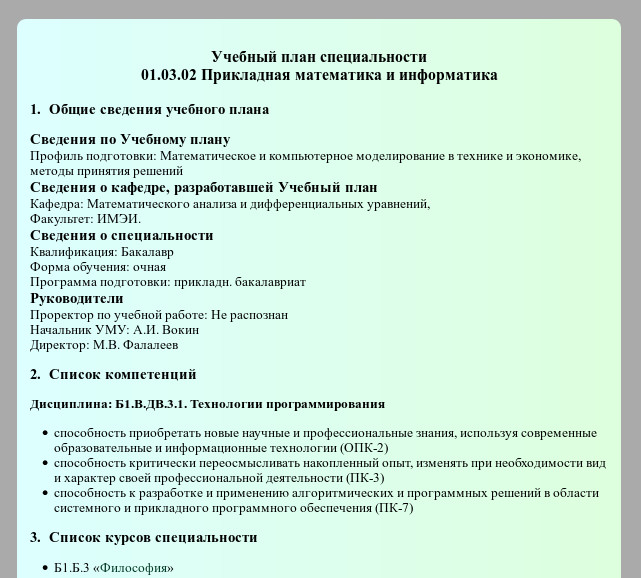
\includegraphics[width=0.7\linewidth]{template-courses.jpg}
    \end{center}
  \end{adjustwidth}
\end{frame}
\begin{frame}
  \frametitle{Imported time distribution for lecture, seminary, \ldots}
   \begin{adjustwidth}{-2.5em}{-2.5em}
    \begin{center}
      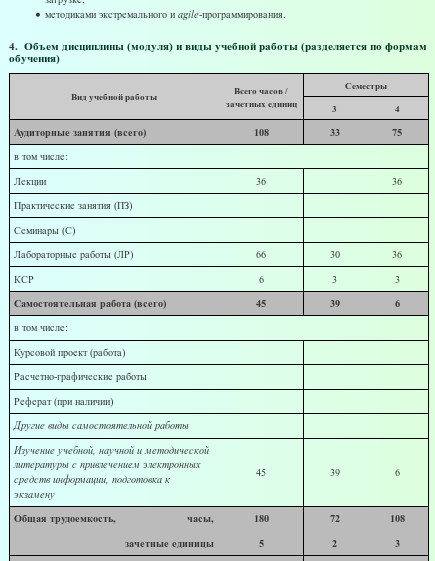
\includegraphics[width=0.9\linewidth]{work-program-volume.jpg}
    \end{center}
  \end{adjustwidth}
\end{frame}

\begin{frame}
  \frametitle{Complete document}
  \begin{adjustwidth}{-2.5em}{-2.5em}
    \begin{center}
      \begin{columns}
        \begin{column}{0.5\linewidth}
          
\includegraphics[width=1\linewidth]{work-program-title.jpg}
        \end{column}
        \begin{column}{0.5\linewidth}
          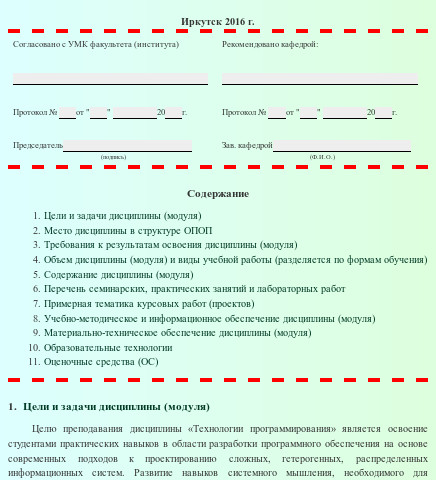
\includegraphics[width=1\linewidth]{work-program-agreement.jpg}
        \end{column}
    \end{columns}
    \end{center}
  \end{adjustwidth}
\end{frame}

\begin{frame}
  \frametitle{Conclusion}
A tools (components) for digital archive implementation, which allows
to device information systems and document processing services
with the following features:
\begin{itemize}
\item load LOD marked up document, extract, store in a graph and index RDF data;
\item retrieve RDF data as triples or as a result of full-text search query;
\item combine existing LOD data and its content in new documents dynamically with browser based context inference machine;
\item use server-site inference machine (Prolog) to process RDF data upon
  request from browser's part of the system;
  % \item organizes a platform for document semantic markup,
\item convert created RDFa marked up HTML5 documents into Excel and Word formats.
\end{itemize}

  \textbf{Applications}
  \begin{itemize}
  \item Document authoring automation;
  \item Context-depended editing;
  % \item Export into office formats;
  \item Self-organizing global document flows;
  \item Documents as data sources for information systems.
  \end{itemize}

\end{frame}

\begin{frame}
  \frametitle{Conclusion}
  The following results have been obtained as for today:
  \begin{itemize}
  \item A technique for model representation has been developed and tested.
  \item A programming technique using object-oriented logical language Logtalk is devised.
  \item Prototypes of various transformation procedures are implemented.
  \item Transformation tools are tested in application areas and no significant technical problems were mentioned.
  \end{itemize}
  Further development directions are as follows:
  \begin{itemize}
  \item A technique for document automatic markup with vocabulary entities.
  \item A transformation implemenation techniques, minimizing usage of dynamic objects, targeting on macro properties of Logtalk.
  \item Form a toolset out of existing prototypes obeying nowadays software development requirements.
  \end{itemize}
  The source codes are available at \url{https://github.com/isu-enterprise/icc.xmitransform}, \url{https://github.com/eugeneai/icc.mothurpim}.
\end{frame}

\end{document}

%%% Local Variables:
%%% mode: latex
%%% TeX-master: t
%%% End:
